\documentclass[11pt,a4paper]{amsart}

\usepackage[margin=1in]{geometry}
\usepackage{amsmath,amssymb,amsthm,mathtools}
\usepackage[expansion=false]{microtype}
\usepackage{pgfplots}
% compat is pinned deliberately: without it pgfplots warns and may change
% defaults between installed versions.
\pgfplotsset{compat=1.18}
\usepackage[colorlinks=true,linkcolor=black,citecolor=black,urlcolor=black]{hyperref}
\usepackage[nameinlink,capitalize]{cleveref}
\hypersetup{
  pdftitle={Bounded exceptional zeros for polynomial initial conditions in the Forgacs-Tran family},
  pdfauthor={John Shields},
  pdfkeywords={real-rooted polynomial, rational generating function,
    hyperbolic polynomial, zero distribution, exceptional zero,
    coalescing poles, initial conditions}
}
\pdfinfo{
  /ORCID (https://orcid.org/0009-0004-3882-4571)
}

\numberwithin{equation}{section}

\theoremstyle{plain}
\newtheorem{theorem}{Theorem}[section]
\newtheorem{proposition}[theorem]{Proposition}
\newtheorem{lemma}[theorem]{Lemma}
\newtheorem{corollary}[theorem]{Corollary}

\theoremstyle{definition}
\newtheorem{definition}[theorem]{Definition}
\newtheorem{remark}[theorem]{Remark}
\newtheorem{question}[theorem]{Question}

\newcommand{\R}{\mathbb R}
\newcommand{\C}{\mathbb C}
\newcommand{\dd}{\,\mathrm d}

\title[Bounded exceptional zeros in the Forg\'acs--Tran family]
{Bounded exceptional zeros for polynomial\\
initial conditions in the Forg\'acs--Tran family}

\author{John Shields}
\date{July 28, 2026}
\thanks{Independent researcher, Ginza 2-15-2, KR Ginza II 5F, Chuo-ku, Tokyo,
Japan 104-0061.  Corresponding author:
\href{mailto:math@johnnyshields.com}{math@johnnyshields.com}.
ORCID: \href{https://orcid.org/0009-0004-3882-4571}{0009-0004-3882-4571}.
This work is archived at
\href{https://doi.org/10.5281/zenodo.21517117}{doi:10.5281/zenodo.21517117}.}

\subjclass[2020]{Primary 26C10; Secondary 05A15, 30C15}
\keywords{real-rooted polynomial, rational generating function, hyperbolic polynomial,
zero distribution, exceptional zero, coalescing poles, initial conditions}

\begin{document}

\begin{abstract}
Let \(Q\in\R[t]\) be nonconstant with \(Q(0)>0\) and only positive real zeros,
fix \(r\ge1\) with \(\max\{\deg Q,r\}>1\) and a numerator
\(N\in\R[t,z]\setminus\{0\}\) with \(\deg_tN<\deg_t(Q+zt^r)\), and
define \(P_m(z)\) by \(N(t,z)/(Q(t)+zt^r)=\sum_{m\ge0}P_m(z)t^m\).  The
denominator determines a linear recurrence and \(N\) its polynomial initial
conditions; for \(N=1\), Forg\'acs and Tran proved every sufficiently large
\(P_m\) real-rooted, with all zeros in an explicit interval
\(I_{Q,r}\subset(0,\infty)\).  They ask whether the number of zeros of
\(P_m\) outside \((0,\infty)\) admits a bound depending only on \(r\) and
\(\deg Q\).  We prove that for each fixed \(N\) there is a constant
\(C=C(Q,r,N)\) such that every nonzero \(P_m\) has at most \(C\) zeros outside
\((0,\infty)\), counted with multiplicity, and every sufficiently large \(P_m\)
at most \(C\) outside \(I_{Q,r}\).  The latter have at least
\(\deg P_m-C\) distinct zeros in \(I_{Q,r}\), and
\(\deg P_m=m/r+O_{Q,r,N}(1)\), so arbitrary fixed polynomial initial
conditions cost the positive-real bulk only a bounded
defect.  Normalized by degree, the zero-counting measures converge weakly to
the pushforward of uniform angular measure under the Forg\'acs--Tran
parameterization, the same limit for every fixed numerator.  Neither the
defect nor the dependence of \(C\) on \(N\) can be removed: a numerator
\(R(z)\) forces arbitrarily many negative, hence exceptional, zeros into
every nonzero \(P_m\).
\end{abstract}

\maketitle

\section{Introduction}\label{sec:introduction}

The zeros of polynomial sequences defined by rational generating functions
are often controlled by the relative moduli of the denominator roots.  That
their limiting loci are governed by competition between dominant denominator
roots and by the vanishing of the associated residue amplitudes goes back to
Beraha, Kahane, and Weiss \cite{Beraha1975} and, in the general form of
competing analytic branches \(\sum_k\alpha_k(z)\beta_k(z)^m\), to
Sokal \cite[Thm.~1.5]{Sokal2004}; for coefficient sequences of rational generating
functions it was developed by Tran \cite{Tran2014,Tran2015}.  Forg\'acs and
Tran introduced the following positive-rooted family.  Let
\(Q\in\R[t]\) satisfy
\begin{equation}\label{eq:Q-hypotheses}
 Q(0)>0,
 \qquad
 Q(t)=Q(0)\prod_{j=1}^{n}\left(1-\frac{t}{x_j}\right),
 \qquad
 0<x_1\le\cdots\le x_n,
\end{equation}
where multiplicities are allowed, and let \(r\ge1\).  The denominator-only
sequence
\begin{equation}\label{eq:H-generating}
 \frac1{Q(t)+zt^r}=\sum_{m\ge0}H_m(z)t^m
\end{equation}
was shown by Forg\'acs and Tran to be eventually hyperbolic---every
sufficiently large \(H_m\) real-rooted---with all zeros lying in an explicitly
determined interval \(I_{Q,r}=(a,b)\subset(0,\infty)\) \cite{Forgacs2017}.  Their proof constructs a strictly monotone
parameterization \(z=z(\theta)\), \(0<\theta<\pi/r\), for which the two
minimum-modulus denominator zeros form the conjugate pair
\[
 t_\pm(\theta)=\tau(\theta)e^{\pm i\theta}.
\]
This pair is called \emph{principal}, the remaining zeros of the denominator
\emph{nonprincipal}.
The coefficient \(H_m(z(\theta))\) is then governed by the interference of
these two modes.  Estimates near both endpoints show that the resulting
phase produces at least \(\lfloor m/r\rfloor\) positive zeros, the maximum
permitted by the degree.

In Problem~14 of their earlier paper \cite{Forgacs2016}, Forg\'acs and Tran
asked what remains true when the numerator is allowed to vary.  There one fixes
a real bivariate polynomial \(N(t,z)\) with
\[
 \deg_tN<\deg_t(Q(t)+zt^r)
\]
and defines
\begin{equation}\label{eq:P-generating-intro}
 \frac{N(t,z)}{Q(t)+zt^r}=\sum_{m\ge0}P_m(z)t^m.
\end{equation}
They ask whether the number of zeros of \(P_m\) outside \((0,\infty)\) is
bounded independently of \(m\).  As printed, the
constant depends at most on \(r\) and \(\deg Q\), hence must be uniform over
the numerator.  The surrounding discussion, however, treats the numerator as
the fixed initial conditions for the denominator recurrence: there ``the denominator
of the generating function gives the recurrence relation for \(P_m(z)\) whereas
the numerator gives rise to the set of initial polynomials'', an equivalence
made precise in \Cref{prop:initial-data}.  On the same page the problem is
also rephrased as showing that the \(P_m\) have zero loci similar to those of the
sequence generated by \(1/(Q(t)+zt^r)\), after \cite{Goh2009}; that gloss is the
asymptotic reading, settled by \Cref{prop:equidistribution}.  The theorem below
treats the fixed-numerator regime,
with \(N\) held fixed as \(m\to\infty\) rather than varying with the index.

The dependence on \(N\) cannot be omitted.  If \(R(z)\in\R[z]\) and
\(N(t,z)=R(z)\), then
\[
 P_m(z)=R(z)H_m(z),
\]
so the fixed zeros of \(R\) occur in every coefficient polynomial.  Any bound
on the exceptional zeros must therefore depend on \(N\), giving \(C=C(Q,r,N)\)
and showing that no uniform-in-\(N\) bound is possible; see \Cref{prop:N-dependence}.

The question is one of stability under a change of initial conditions.  The
denominator \(Q(t)+zt^r\) fixes the recurrence and its pole geometry, while
\(N\) fixes the initial conditions; eventual hyperbolicity for the single numerator
\(N=1\) need not persist when that data changes.  \Cref{thm:main}
shows that it persists with only a bounded loss: arbitrary fixed polynomial
initial conditions can create exceptional zeros, but only \(O(1)\) of them.  The
asymptotic positive-real zero bulk and its containing interval are therefore
determined by the denominator alone.
The normalized zero-counting measures converge weakly to a single limit, the
same for every fixed numerator (\Cref{prop:equidistribution}).
Beraha--Kahane--Weiss theory \cite{Beraha1975,Sokal2004} identifies the loci
where the zeros accumulate but gives no bound on the number lying away
from them at finite degree; the present theorem supplies that bound, uniformly
in \(m\).

Tran noted that his zero-location theorem for polynomials with a three-term
recurrence persists for a monomial numerator in \(t\) and \(z\), and reported
unpublished work with Boyer that a general numerator sends the zeros toward the
curve of that theorem up to a possible finite exceptional set
\cite[p.~879]{Tran2015}.  That indication is
asymptotic, a statement about the limiting zero set, whereas \Cref{thm:main}
bounds the exceptional zeros of each \(P_m\) uniformly in \(m\), for the
positive-rooted pencil and with the explicit interval \(I_{Q,r}\).

For polynomials satisfying
a three-term recurrence, Mai bounded the number of zeros that leave the
recurrence's limiting curve under initial conditions more general than the
canonical one: for the family
\(\bigl(aB(z)t+b\bigr)/\bigl(1+B(z)t+A(z)t^2\bigr)\), whose letters are his and
unrelated to those used here, he obtained at most
\(\max\{\deg A,2\deg B\}\) such zeros, uniformly in the index \cite[Thm.~1]{Mai2018}.
The same phenomenon, finitely many exceptional zeros created by a change of
initial conditions, occurs here in a complementary setting.  There the
recurrence is of second order and the initial conditions available there form the
two-parameter family \(P_0=b\), \(P_1=(a-b)B\), and the limiting locus may be a
complex curve; here the denominator is the positive-rooted pencil
\(Q(t)+zt^r\) of arbitrary order, the initial conditions are arbitrary
(\Cref{prop:initial-data}), and the locus is the real interval \(I_{Q,r}\).

Bounds of this kind are known for other fixed pencils.  For the doubly indexed
family generated by \(\widetilde N(s,t,z)/(1+s+t+zst)\), where the numerator likewise
supplies the initial polynomials, Luong and Tran bounded the number of nonreal
zeros by \(\deg_s\widetilde N+\deg_t\widetilde N+2\deg_z\widetilde N\)
\cite{Luong2022}.  Al Hamdani and Tran treated
\(1/\bigl((1-t)^\alpha(1-2zt+t^2)\bigr)\) with \(0<\alpha<1\) and bounded the
number of zeros outside \((-1,1)\) by a constant independent of the index
\cite{AlHamdani2022}, by a conjugate-pair extraction and phase count of the
same shape as the argument below.  Neither denominator is of the form
\(Q(t)+zt^r\) with \(Q\) positive-rooted, and neither bound contains or is
contained in \Cref{thm:main}: the pencil fixed here is the one of Problem~14,
and the zeros are counted off the positive ray rather than off \(\R\) or off a
fixed interval.

The main theorem is the following.

\begin{theorem}[Fixed-numerator Forg\'acs--Tran theorem]\label{thm:main}
Let \(Q\in\R[t]\) be nonconstant and satisfy \eqref{eq:Q-hypotheses}.  Let
\(r\ge1\) and assume
\[
 \max\{\deg Q,r\}>1.
\]
Let \(N\in\R[t,z]\setminus\{0\}\) satisfy
\[
 \deg_tN<\deg_t(Q(t)+zt^r),
\]
where \(\deg_t\) is the degree in \(t\) over \(\R[z]\), so that
\(\deg_t(Q(t)+zt^r)=\max\{\deg Q,r\}\).
Define \(P_m\in\R[z]\) by \eqref{eq:P-generating-intro}.  Then there exists
\(C=C(Q,r,N)\) such that every nonzero \(P_m\) has at most \(C\) zeros outside
\((0,\infty)\), counted with multiplicity.

More precisely, if \(I_{Q,r}=(a,b)\) is the Forg\'acs--Tran interval defined in
\eqref{eq:ab-def}, then every sufficiently large \(P_m\) is nonzero, has at
most \(C\) zeros outside \(I_{Q,r}\), counted with multiplicity, and has at least
\(\deg P_m-C\) distinct zeros in \(I_{Q,r}\).
\end{theorem}

Br\"and\'en and Leite have since proved all-degree real-rootedness
and interlacing for the de\-nom\-i\-na\-tor-only family through total nonnegativity
\cite[Thm.~4.5]{Branden2026}, settling Problem~13 of Forg\'acs and Tran
\cite{Forgacs2016} for \(r\ge1\).  Their parameter is the negative of \(z\), and
the zeros they obtain
are negative, so for every \(Q\) satisfying \eqref{eq:Q-hypotheses} the
conclusion is real-rootedness together with containment in \((0,\infty)\) rather
than real-rootedness alone.  That family is the case \(N=1\); the
present theorem concerns arbitrary fixed initial conditions, where the numerator
may force nonreal or nonpositive zeros.  The conclusion here is that this
failure is confined to a bounded defect.

The excluded case \(\deg Q=r=1\) is elementary and satisfies the first
conclusion of \Cref{thm:main}, the second being vacuous there; see
\Cref{prop:linear-case}.  The hypothesis \(r\ge1\) is
essential to the polynomial formulation: for \(r=0\), the coefficients are
generally rational rather than polynomial functions of \(z\).  We also
exclude constant \(Q\), for which \(P_m\) may have a zero of large multiplicity
at the origin.  Apart from \Cref{prop:linear-case}, the hypotheses
\eqref{eq:Q-hypotheses} and \(\max\{\deg Q,r\}>1\) are in force throughout; a
denominator \(Q(t)+zt^r\) meeting them is called \emph{admissible}.  The
latter gives \(rQ(t)-tQ'(t)\) a positive zero, hence \(t_a\), and at \(r=1\) forces
\(\deg Q\ge2\) and with it the negative zero \(t_b\), so that \(I_{Q,r}\) exists; at
\(\deg Q=r=1\) that polynomial reduces to the nonzero constant \(Q(0)\).

The proof has four components.  \Cref{sec:reduction} reduces, by an exact
division in the Laurent polynomial ring, an arbitrary bivariate numerator to
a fixed univariate numerator \(B(t)\) with \(B(0)\ne0\) at the cost of a finite
index shift \(m\mapsto M=m+O(1)\), and establishes the eventual degree formula
\[
 \deg [t^M]\frac{B(t)}{Q(t)+zt^r}=\left\lfloor\frac Mr\right\rfloor.
\]
\Cref{sec:geometry} records the denominator geometry imported from Forg\'acs
and Tran and the principal-pair decomposition; the univariate numerator
enters only through the amplitude \(B(t_+(\theta))\), which has finitely many
zeros on the branch and phase of bounded variation
(\Cref{lem:amplitude-divisor}).

\Cref{sec:dominance} extends the three-region estimates of
\cite[Prop.~3]{Forgacs2017} to this weighted amplitude:
away from the two endpoints and from small neighborhoods of the amplitude
zeros, the principal conjugate pair dominates, and truncating angular windows
of width \(O(1/M)\) costs only \(O(1)\) phase oscillations.  \Cref{sec:proof} counts
the sign changes of the resulting phase, giving \(\lfloor M/r\rfloor-O(1)\)
distinct zeros in \(I_{Q,r}\); the eventual degree formula completes the proof.

\section{Laurent reduction and eventual degree}\label{sec:reduction}

Throughout the paper, put
\[
 D(t,z)=Q(t)+zt^r,
 \qquad
 d=\deg_tD=\max\{\deg Q,r\}.
\]
The numerator carries the same information as the initial conditions of the
denominator recurrence.

\begin{proposition}\label{prop:initial-data}
Write \(D(t,z)=\sum_{j=0}^d d_j(z)t^j\), so that \(d_0=Q(0)\ne0\).  For each
\(N=\sum_{m=0}^{d-1}N_m(z)t^m\) with \(N_m\in\R[z]\), the coefficients \(P_m\) of
\(N/D\) satisfy
\[
 \sum_{j=0}^{m}d_j(z)P_{m-j}(z)=N_m(z)
 \qquad(0\le m<d).
\]
This is a lower-triangular system with constant diagonal \(d_0=Q(0)\), so
\(N\mapsto(P_0,\dots,P_{d-1})\) is a bijection from proper numerators, those with
\(\deg_tN<d\), onto
\(\R[z]^d\).  A fixed proper \(N\) is thus the same datum as a fixed vector
\((P_0,\dots,P_{d-1})\) of polynomial initial conditions.
\end{proposition}

\begin{proof}
Equating coefficients of \(t^m\) in \(N=D\sum_{k\ge0}P_kt^k\) gives the displayed
equations for \(0\le m<d\) and \(\sum_{j=0}^d d_j(z)P_{m-j}(z)=0\) for \(m\ge d\).
The first \(d\) equations express \((N_0,\dots,N_{d-1})\) from
\((P_0,\dots,P_{d-1})\) by a lower-triangular matrix with constant diagonal
\(d_0=Q(0)\ne0\), invertible over \(\R[z]\); the remaining equations then
determine \(P_m\) for \(m\ge d\).
\end{proof}

The following reduction uses the linearity of \(D\) in \(z\) together with the fact
that its \(z\)-coefficient \(t^r\) is a unit in the Laurent polynomial ring
\(\R[t,t^{-1}]\).

\begin{lemma}[Laurent--Gauss reduction]\label{lem:laurent-reduction}
Let \(N\in\R[t,z]\setminus\{0\}\) satisfy \(\deg_tN<d\), and set
\(E=\deg_zN\).  Define
\begin{equation}\label{eq:A-def}
 A(t)=t^{rE}N\!\left(t,-\frac{Q(t)}{t^r}\right).
\end{equation}
Then \(A\in\R[t]\setminus\{0\}\).  There is an
\(S\in\R[t,t^{-1},z]\) such that
\begin{equation}\label{eq:laurent-division}
 N(t,z)=D(t,z)S(t,z)+t^{-rE}A(t).
\end{equation}
If \(A(t)=t^\mu B(t)\) with \(B(0)\ne0\), then for all sufficiently large \(m\),
\begin{equation}\label{eq:reduction-coeff}
 P_m(z)=[t^{m+rE-\mu}]\frac{B(t)}{D(t,z)}.
\end{equation}
\end{lemma}

\begin{proof}
Write
\[
 N(t,z)=\sum_{\alpha,\beta}c_{\alpha,\beta}t^\alpha z^\beta.
\]
After the substitution in \eqref{eq:A-def}, the corresponding term is
\[
 c_{\alpha,\beta}(-1)^\beta
 t^{\alpha+r(E-\beta)}Q(t)^\beta,
\]
which is a polynomial in \(t\).  Thus \(A\in\R[t]\).

Suppose that \(A\equiv0\).  Then, as a polynomial in \(z\) over the field
\(\R(t)\),
\[
 N\!\left(t,-\frac{Q(t)}{t^r}\right)=0.
\]
Since \(D(t,z)\) is linear in \(z\), it follows that \(D\) divides \(N\) in
\(\R(t)[z]\).  The polynomials \(Q(t)\) and \(t^r\) are coprime because \(Q(0)\ne0\),
so \(D\) is primitive in \(\R[t][z]\).  Gauss's lemma gives \(D\mid N\) in
\(\R[t,z]\).  Since \(\R[z][t]\) is an integral domain,
\[
 \deg_tN\ge\deg_tD=d,
\]
a contradiction.  Hence \(A\ne0\).

In the Laurent ring \(\R[t,t^{-1}][z]\), the polynomial
\[
 N(t,z)-t^{-rE}A(t)
\]
vanishes at \(z=-Q(t)/t^r\).  Since \(z+Q(t)/t^r\) is monic in \(z\), the factor
theorem gives divisibility by \(z+Q(t)/t^r\) in \(\R[t,t^{-1}][z]\); and since
\(t^r\) is a unit in \(\R[t,t^{-1}]\), divisibility by \(D=t^r(z+Q/t^r)\) follows,
with a Laurent-polynomial quotient.  This proves \eqref{eq:laurent-division}.

Divide \eqref{eq:laurent-division} by \(D\).  Since \(S\) is a Laurent
polynomial, it contains only finitely many powers of \(t\).  For all sufficiently
large \(m\), its \(t^m\) coefficient vanishes, and therefore
\[
 P_m(z)=[t^{m+rE}]\frac{A(t)}{D(t,z)}.
\]
Factoring \(A=t^\mu B\) gives \eqref{eq:reduction-coeff}.
\end{proof}

For all sufficiently large \(m\), writing \(B(t)=\sum_jb_jt^j\) and expanding
\eqref{eq:reduction-coeff} against \eqref{eq:H-generating} exhibits the
reduced coefficient as a fixed finite linear combination of the
denominator-only sequence,
\begin{equation}\label{eq:P-linear-combination}
 P_m(z)=\sum_jb_jH_{m+rE-\mu-j}(z),
\end{equation}
with coefficients independent of \(m\).

Thus the proof reduces to one fixed univariate numerator.  Throughout, let
\begin{equation}\label{eq:F-M-def}
 F_M(z)=[t^M]\frac{B(t)}{Q(t)+zt^r},
 \qquad B\in\R[t],\quad B(0)\ne0.
\end{equation}

\begin{lemma}\label{lem:eventual-degree}
For all sufficiently large \(M\),
\begin{equation}\label{eq:eventual-degree}
 \deg F_M=\left\lfloor\frac Mr\right\rfloor.
\end{equation}
\end{lemma}

\begin{proof}
The geometric expansion
\begin{equation}\label{eq:geometric-expansion}
 \frac{B(t)}{Q(t)+zt^r}
 =\sum_{j\ge0}(-z)^jt^{rj}\frac{B(t)}{Q(t)^{j+1}}
\end{equation}
gives
\begin{equation}\label{eq:F-coefficient-expansion}
 F_M(z)=\sum_{0\le j\le M/r}(-z)^j
 [t^{M-rj}]\frac{B(t)}{Q(t)^{j+1}}.
\end{equation}
Hence \(\deg F_M\le\lfloor M/r\rfloor\).

Put
\[
 \ell=\left\lfloor\frac Mr\right\rfloor,
 \qquad
 s=M-r\ell,
 \qquad 0\le s<r.
\]
The coefficient of \(z^\ell\) is
\begin{equation}\label{eq:leading-z-coeff}
 (-1)^\ell[t^s]\frac{B(t)}{Q(t)^{\ell+1}}.
\end{equation}
Let
\[
 \lambda=-\frac{Q'(0)}{Q(0)}=\sum_{j=1}^n\frac1{x_j}>0.
\]
For each fixed \(s\), expanding
\(Q(t)^{-(\ell+1)}=Q(0)^{-(\ell+1)}\prod_{j=1}^n(1-t/x_j)^{-(\ell+1)}\) and
extracting the coefficient of \(t^s\) shows that
\[
 Q(0)^{\ell+1}\,[t^s]\frac{B(t)}{Q(t)^{\ell+1}}
\]
is a polynomial in \(\ell\) of degree at most \(s\), with leading coefficient
\(B(0)\lambda^s/s!\).  Since \(B(0)\lambda^s\ne0\), it does not vanish
identically and is therefore nonzero for all sufficiently large \(\ell\), so the
upper bound on the degree is attained.
\end{proof}

\begin{remark}\label{rem:degree-shift}
The shift \(M=m+rE-\mu\) in \Cref{lem:laurent-reduction} is fixed.  Thus
\[
 \deg P_m=\frac mr+O_{Q,r,N}(1)
\]
eventually.
\end{remark}

\section{Pole geometry and the weighted principal amplitude}\label{sec:geometry}

This section records the denominator facts needed in the weighted argument.  They are
established in \cite{Forgacs2017}, except for the case \((\deg Q,r)=(2,1)\), a
quadratic denominator excluded there because \(\tau\) is then constant; that case
is elementary and is recorded in \Cref{rem:quadratic-case}.  The linear modulus
gap \eqref{eq:endpoint-linear-gap} is derived below.
\Cref{lem:cluster-safe,lem:degree-drop,lem:amplitude-divisor} then group the
nonprincipal roots by a fixed contour, treat an escaping root, and give the
endpoint form and phase bound for the weighted principal amplitude \(W\) of
\eqref{eq:W-def}; \Cref{sec:dominance,sec:proof} consume all three.

Let
\[
 g(t)=-\frac{Q(t)}{t^r}.
\]
Following Forg\'acs and Tran, let \(t_a>0\) be the smallest positive critical
point of \(g\), and set \(b=+\infty\) when \(r>1\), while for \(r=1\) let \(t_b<0\) be
the unique negative critical point of \(g\) \cite[Lem.~5]{Forgacs2017} and put
\(b=g(t_b)\).  This is the endpoint convention of \cite[Thm.~1]{Forgacs2017},
where both endpoints are read off the polynomial
\(t^{r-1}\bigl(rQ(t)-tQ'(t)\bigr)\); its zero of order \(r-1\) at the origin is
what makes the upper endpoint unbounded for \(r>1\).
Set
\begin{equation}\label{eq:ab-def}
 a=g(t_a),
 \qquad
 I_{Q,r}=(a,b).
\end{equation}

\begin{theorem}[Forg\'acs--Tran denominator geometry]\label{thm:FT-geometry}
There are real-analytic functions
\[
 \tau:(0,\pi/r)\to(0,\infty),
 \qquad
 z:(0,\pi/r)\to I_{Q,r},
\]
with \(z\) strictly increasing, \(z(\theta)\to a\) as \(\theta\downarrow0\) and
\(z(\theta)\to b\) as \(\theta\uparrow\pi/r\), such that
\begin{equation}\label{eq:principal-pair}
 t_\pm(\theta)=\tau(\theta)e^{\pm i\theta}
\end{equation}
are zeros of \(Q(t)+z(\theta)t^r\).  They are the only denominator zeros in
the closed disk \(|t|\le\tau(\theta)\).

On every compact subinterval of \((0,\pi/r)\), the remaining denominator
zeros are separated from the principal pair by a uniform modulus ratio.
Near each endpoint, write \(\zeta_j(\theta)=t_j(\theta)/\tau(\theta)\) for the
normalized denominator zeros.  At \(\theta\downarrow0\), a smallest zero \(x_1\)
of \(Q\) of multiplicity \(\rho\ge2\) produces a cluster of \(\rho\) zeros tending
to \(x_1\), whose \(\rho-2\) nonprincipal members satisfy a linear modulus
gap
\begin{equation}\label{eq:endpoint-linear-gap}
 |\zeta_j(\theta)|\ge1+c\delta,
\end{equation}
for some \(c>0\), \(\delta\) denoting the angular distance to the endpoint, while
every zero outside the cluster satisfies
\begin{equation}\label{eq:endpoint-fixed-gap}
 |\zeta_j(\theta)|\ge1+c_*
\end{equation}
for a fixed \(c_*>0\).  When \(\rho=1\) the cluster is the principal pair alone
and every nonprincipal zero satisfies \eqref{eq:endpoint-fixed-gap}.  At
\(\theta\uparrow\pi/r\) with \(r>1\), the finite normalized cluster approaches the
\(r\)th roots of \(-1\) and its nonprincipal members satisfy
\eqref{eq:endpoint-linear-gap}, while every other normalized zero tends to
infinity.  At \(\theta\uparrow\pi\) with \(r=1\), the principal pair coalesces at
\(t_b\) to a zero of multiplicity exactly two, and every other normalized zero
satisfies \eqref{eq:endpoint-fixed-gap}.
\end{theorem}

\begin{proof}
The existence, strict monotonicity, and endpoint limits of \(\tau\) and \(z\)
are established in Lemmas~2--6 of \cite{Forgacs2017}.
The minimum-modulus assertion is
\cite[Props.~1--2]{Forgacs2017}.  Both exclude \((\deg Q,r)=(2,1)\), where
\(\tau\) is constant; that case is \Cref{rem:quadratic-case}.  Compact-uniform
separation follows by continuity of the roots, compactness, and the strict
pointwise modulus gap.

The endpoint statement is the quantitative content of the second and third
cases in the proof of \cite[Prop.~3]{Forgacs2017}.  At the lower
endpoint, a smallest zero of multiplicity \(\rho\ge2\) gives normalized cluster
roots
\[
 \zeta_j(\theta)=1+\frac{\cos(\pi/\rho)-\omega_j}{\sin(\pi/\rho)}\,\theta
 +O(\theta^2),\qquad\omega_j=e^{(2j-1)\pi i/\rho},
\]
so that
\[
 |\zeta_j(\theta)|=1+\frac{\cos(\pi/\rho)-\Re\omega_j}{\sin(\pi/\rho)}\,\theta
 +O(\theta^2);
\]
the linear coefficient vanishes exactly for the two principal indices
\(\omega_j=e^{\pm i\pi/\rho}\) and is strictly positive otherwise.  At the upper
endpoint for \(r>1\), with \(\eta=\pi/r-\theta\) and \(\omega_j\) now the \(r\)th roots of
\(-1\),
\[
 |\zeta_j(\theta)|=1+\frac{\cos(\pi/r)-\Re\omega_j}{\sin(\pi/r)}\,\eta+O(\eta^2),
\]
again with vanishing linear coefficient only for the principal pair
\(\omega_j=e^{\pm i\pi/r}\).  Since the clusters are finite, the positive linear
coefficients have a uniform positive minimum and the remainders are uniform
over the cluster, giving \eqref{eq:endpoint-linear-gap}.  For \(\rho=2\) the
cluster is the principal pair alone and
\eqref{eq:endpoint-linear-gap} is vacuous.

The zeros outside the cluster keep a fixed gap.  At the lower endpoint
\(\tau(\theta)\to t_a\) and \(z(\theta)\to a\); among the zeros of
\(Q(t)+z(\theta)t^r\) that remain bounded, the normalized values converge to the
zeros of the limit polynomial obtained at \((\tau,z)=(t_a,a)\), namely \(\zeta=1\)
with multiplicity \(\max\{\rho,2\}\) together with the ratios \(t_j/t_a\) formed
from the remaining bounded zeros \(t_j\) of \(Q(t)+at^r\), each of modulus
exceeding \(t_a\).  The minimum-modulus assertion is quantified over
\(\theta\in(0,\pi/r)\) and in the limit gives only \(|t_j|\ge t_a\), so strictness
is supplied directly.  Let \(t_e\ne0\) and \(z_e\) be real with
\(Q(t_e)+z_et_e^{r}=0\).  For
\(|t|=|t_e|\) with \(t\ne t_e\) one has \(\Re t<t_e\) if \(t_e>0\) and
\(\Re t>t_e\) if \(t_e<0\), so
\[
 |t-x_j|^2-|t_e-x_j|^2=2x_j(t_e-\Re t)
 \qquad(1\le j\le n)
\]
has the sign of \(t_e\) for every \(j\); hence
\(|Q(t)|\ne|Q(t_e)|=|z_e|\,|t_e|^{r}=|z_et^{r}|\) and \(t\) is not a zero of
\(Q(t)+z_et^{r}\) \cite[Prop.~3]{Forgacs2017}.  At the lower endpoint this
applies with \(t_e=t_a\) and \(z_e=a\).  For \(\rho\ge2\), both \(Q\) and
\(Q'\) vanish at \(x_1\), so \(x_1\) is a critical point of \(g\); as
\(tQ'(t)-rQ(t)<0\) on \((0,x_1)\), it is the smallest positive one.  Hence
\(t_a=x_1\) and \(a=g(x_1)=-Q(x_1)/x_1^{r}=0\), so the limit polynomial is
\[
 Q(0)(1-\zeta)^{\rho}\prod_{j>\rho}\left(1-\frac{x_1\zeta}{x_j}\right),
\]
whose zeros off \(\zeta=1\) are the fixed ratios \(x_j/x_1>1\).  Continuity of the
zeros in the coefficients gives \eqref{eq:endpoint-fixed-gap} for any \(c_*\)
below the least of these ratios diminished by one.

At the upper endpoint for \(r=1\) the comparison above applies with
\(t_e=t_b<0\) and \(z_e=b\), the sign in the display reversing with \(t_e\).  A
multiplicity above two at \(t_b\) would force \(Q''(t_b)=0\), whereas the zeros of
\(Q''\) are positive; the collision is therefore exactly double, and
\(\deg Q\ge2>r\) leaves no escaping zero, the leading \(t\)-coefficient of
\(Q(t)+zt\) being the nonzero constant \(q_{\deg Q}\), so the
remaining \(\deg Q-2\) zeros satisfy \eqref{eq:endpoint-fixed-gap} by continuity
of the zeros in the coefficients \cite[Prop.~3]{Forgacs2017}.  The zeros that escape to
infinity are treated in \Cref{lem:degree-drop} and in the proof of
\Cref{thm:weighted-dominance}.  The upper endpoint for \(r>1\) is the third case
of the same proof, where the normalized zeros outside the finite cluster tend
to infinity.
\end{proof}

\begin{remark}\label{rem:quadratic-case}
For \(\deg Q=2\) and \(r=1\), write \(Q(t)=q_0+q_1t+q_2t^2\), so that \(q_0,q_2>0\) and
\(q_1<0\).  The two zeros of \(Q(t)+zt\) have product \(q_0/q_2\), so the conjugate
pair \eqref{eq:principal-pair} has \(\tau=\sqrt{q_0/q_2}\), constant in \(z\), and
\[
 z(\theta)=-q_1-2\sqrt{q_0q_2}\,\cos\theta
 \qquad(0<\theta<\pi),
\]
which is real-analytic and strictly increasing, with
\(t_{a}=\sqrt{q_0/q_2}=-t_b\) and \(I_{Q,r}=(-q_1-2\sqrt{q_0q_2},\,
-q_1+2\sqrt{q_0q_2})\).  The pair exhausts the zeros of the denominator, so the
minimum-modulus assertion is immediate, the collision at either endpoint is
exactly double, and \eqref{eq:endpoint-linear-gap} and
\eqref{eq:endpoint-fixed-gap} are vacuous.
\end{remark}

As \(z\) is a strictly monotone bijection onto \(I_{Q,r}\), its inverse is written
\(\theta(z)\), and \(\tau(z)\) abbreviates \(\tau(\theta(z))\).

The coefficient asymptotics are easiest away from multiple denominator
roots.  If \(t_1,\ldots,t_d\) are the simple roots of \(Q(t)+zt^r\), then for
every \(M>\deg B-d\)
\begin{equation}\label{eq:partial-fraction-coefficient}
 F_M(z)=-\sum_{j=1}^d
 \frac{B(t_j)}{t_j^{M+1}\bigl(Q'(t_j)+rz t_j^{r-1}\bigr)},
\end{equation}
the polynomial part of \(B/(Q+zt^r)\), of \(t\)-degree \(\deg B-d\), contributing
nothing to \([t^M]\) in this range.  At a nonprincipal collision, the
individual terms may be singular even though their sum is regular.  Such roots
are always grouped by a fixed contour.

\begin{lemma}\label{lem:cluster-safe}
Let \(K\) be a compact parameter interval in \(I_{Q,r}\cup\{a\}\), or in
\(I_{Q,r}\cup\{a,b\}\) when \(r=1\), and let
\(\Gamma\) be a contour enclosing a complete cluster of denominator roots and
no other roots for every \(z\) in a neighborhood of \(K\).  Then the contribution
of that cluster to \(F_M(z)\) is holomorphic in \(z\) and equals
\begin{equation}\label{eq:cluster-contour}
 -\frac1{2\pi i}\int_\Gamma
 \frac{B(t)}{t^{M+1}(Q(t)+zt^r)}\dd t.
\end{equation}
If the contour may be chosen in \(|t|\ge R_0>\tau(z)\), then after
multiplication by \(\tau(z)^{M+1}\) the contribution is
\[
 O_K(\sigma^M)
\]
for some fixed \(\sigma<1\).
\end{lemma}

\begin{proof}
The contour integral is invariant under the internal splitting or collision
of the roots and is holomorphic by differentiation under the integral sign.
On \(\Gamma\), where \(|t|\ge R_0\), \(|B(t)|\) is bounded above and \(|Q(t)+zt^r|\) is
bounded below, so the contour estimate bounds the contribution by \(C_KR_0^{-M}\)
with \(C_K\) depending on the length of \(\Gamma\), the upper bound for \(B\), and the
lower bound for the denominator; multiplying by \(\tau(z)^{M+1}\) and using
\(\tau(z)\le\sigma R_0\) with \(\sigma<1\) uniform on \(K\) gives \(O_K(\sigma^M)\).  Only
\(\sup_K\tau<R_0\) is used, which holds at either finite endpoint, where
\(\tau(a)=t_a\) and, for \(r=1\), \(\tau(b)=|t_b|\) are finite.  A finite cover of
the compact interval supplies finitely many such contours.
\end{proof}

\begin{remark}
That the contour of \Cref{lem:cluster-safe} encloses the same cluster for every
\(z\) in a neighborhood of \(K\) follows, for the principal cluster, from the
minimum-modulus theorem of Forg\'acs and Tran, \Cref{thm:FT-geometry}; for a
nonprincipal cluster it follows from continuity of the denominator zeros in
\(z\) together with the separation of that cluster from the others at each
parameter of \(K\).
\end{remark}

For \(0<\theta<\pi/r\), define the weighted principal amplitude
\begin{equation}\label{eq:W-def}
 W(\theta)
 =-\frac{B(t_+(\theta))}
 {Q'(t_+(\theta))+rz(\theta)t_+(\theta)^{r-1}}.
\end{equation}
The denominator in \eqref{eq:W-def} equals \(-t_+(\theta)^{r}g'(t_+(\theta))\),
since \(z(\theta)=-Q(t_+)/t_+^{r}\) and \(tQ'(t)-rQ(t)=-t^{r+1}g'(t)\).  A
double principal root would make \(t_+(\theta)\) a critical point of \(g\), that is,
would force \(t_+Q'(t_+)=rQ(t_+)\).  This cannot occur.  The zeros of \(Q\) are
positive, so \(Q\) does not vanish off the real axis, and with \(x_1,\dots,x_n\) as
in \eqref{eq:Q-hypotheses}, listed with multiplicity,
\[
 \Im\frac{tQ'(t)}{Q(t)}
 =\Im\sum_{j=1}^n\frac t{t-x_j}
 =-\Im t\sum_{j=1}^n\frac{x_j}{|t-x_j|^2}
 <0
 \qquad(\Im t>0),
\]
whereas \(r\) is real.  Since \(t_+(\theta)=\tau(\theta)e^{i\theta}\) with
\(0<\theta<\pi/r\le\pi\) lies in the open upper half-plane, \(g'(t_+(\theta))\ne0\)
for every such \(\theta\), and \(W\) is finite and real-analytic on \((0,\pi/r)\).
Combining the two conjugate terms in
\eqref{eq:partial-fraction-coefficient} gives
\begin{equation}\label{eq:principal-decomposition}
 \tau(\theta)^{M+1}F_M(z(\theta))
 =2\Re\!\left(W(\theta)e^{-i(M+1)\theta}\right)+R_M(\theta),
\end{equation}
where \(R_M\) is the grouped normalized contribution of every
nonprincipal root.  \Cref{fig:decomposition-and-defect}(A) shows the
decomposition for one numerator.

% Generated by scripts/make_figure_pole_geom.py -- do not edit by hand.
\begin{figure}[p]
\centering
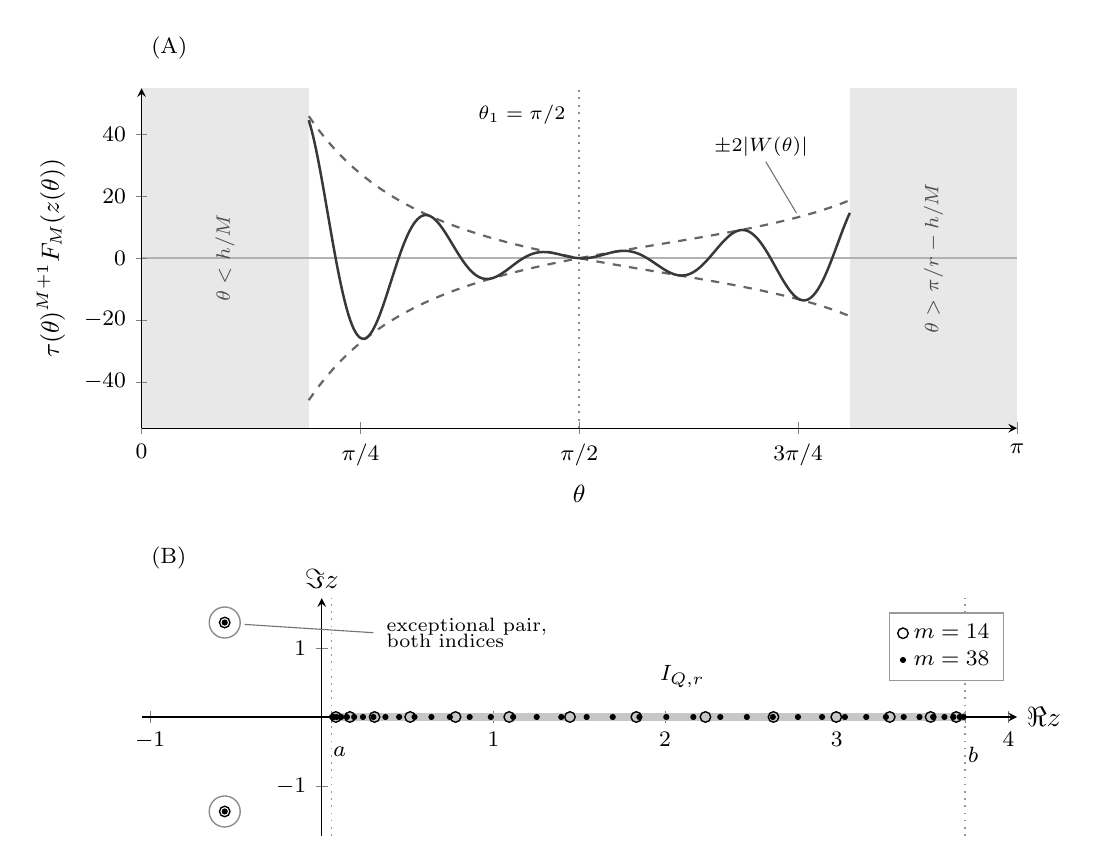
\begin{tikzpicture}
\begin{axis}[
    name=panelA,
    width=12.7cm, height=5.9cm,
    xlabel={\(\theta\)}, ylabel={\(\tau(\theta)^{M+1}F_M(z(\theta))\)},
    xmin=0, xmax=3.1415926536, ymin=-55.00, ymax=55.00,
    xtick={0,0.7853981634,1.5707963268,2.3561944902,3.1415926536},
    xticklabels={\(0\),\(\pi/4\),\(\pi/2\),\(3\pi/4\),\(\pi\)},
    ytick={-40,-20,0,20,40},
    tick label style={font=\footnotesize}, label style={font=\small},
    title={\footnotesize(A)},
    title style={at={(0,1)}, anchor=south west, yshift=1pt},
    axis lines=left, axis on top, clip=true,
]
\fill[black!9] (axis cs:0,-55.00) rectangle (axis cs:0.600000,55.00);
\fill[black!9] (axis cs:2.54159,-55.00) rectangle (axis cs:3.1415926536,55.00);
\addplot[black!30, line width=0.5pt, forget plot]
  coordinates {(0,0) (3.1415926536,0)};
\addplot[black!45, dotted, line width=0.7pt, forget plot]
  coordinates {(1.5707963268,-55.00) (1.5707963268,55.00)};
\addplot[black!60, dashed, line width=0.8pt, forget plot] coordinates {
  (0.600000,45.9360) (0.632360,41.8504) (0.664720,38.1821) (0.697080,34.8754) (0.729440,31.8838) (0.761799,29.1683)
  (0.794159,26.6956) (0.826519,24.4372) (0.858879,22.3688) (0.891239,20.4692) (0.923599,18.7200) (0.955959,17.1053)
  (0.988319,15.6110) (1.02068,14.2247) (1.05304,12.9355) (1.08540,11.7338) (1.11776,10.6110) (1.15012,9.55949)
  (1.18248,8.57232) (1.21484,7.64341) (1.24720,6.76721) (1.27956,5.93874) (1.31192,5.15347) (1.34428,4.40730)
  (1.37664,3.69649) (1.40900,3.01760) (1.44136,2.36750) (1.47372,1.74328) (1.50608,1.14226) (1.53844,0.561948)
  (1.57080,4.37154e-40) (1.60316,0.545775) (1.63552,1.07745) (1.66788,1.59700) (1.70024,2.10632) (1.73260,2.60722)
  (1.76496,3.10149) (1.79732,3.59086) (1.82968,4.07706) (1.86204,4.56180) (1.89440,5.04682) (1.92675,5.53388)
  (1.95911,6.02480) (1.99147,6.52146) (2.02383,7.02584) (2.05619,7.54003) (2.08855,8.06628) (2.12091,8.60699)
  (2.15327,9.16481) (2.18563,9.74262) (2.21799,10.3436) (2.25035,10.9715) (2.28271,11.6302) (2.31507,12.3243)
  (2.34743,13.0592) (2.37979,13.8409) (2.41215,14.6766) (2.44451,15.5746) (2.47687,16.5449) (2.50923,17.5993)
  (2.54159,18.7522)
};
\addplot[black!60, dashed, line width=0.8pt, forget plot] coordinates {
  (0.600000,-45.9360) (0.632360,-41.8504) (0.664720,-38.1821) (0.697080,-34.8754) (0.729440,-31.8838) (0.761799,-29.1683)
  (0.794159,-26.6956) (0.826519,-24.4372) (0.858879,-22.3688) (0.891239,-20.4692) (0.923599,-18.7200) (0.955959,-17.1053)
  (0.988319,-15.6110) (1.02068,-14.2247) (1.05304,-12.9355) (1.08540,-11.7338) (1.11776,-10.6110) (1.15012,-9.55949)
  (1.18248,-8.57232) (1.21484,-7.64341) (1.24720,-6.76721) (1.27956,-5.93874) (1.31192,-5.15347) (1.34428,-4.40730)
  (1.37664,-3.69649) (1.40900,-3.01760) (1.44136,-2.36750) (1.47372,-1.74328) (1.50608,-1.14226) (1.53844,-0.561948)
  (1.57080,-4.37154e-40) (1.60316,-0.545775) (1.63552,-1.07745) (1.66788,-1.59700) (1.70024,-2.10632) (1.73260,-2.60722)
  (1.76496,-3.10149) (1.79732,-3.59086) (1.82968,-4.07706) (1.86204,-4.56180) (1.89440,-5.04682) (1.92675,-5.53388)
  (1.95911,-6.02480) (1.99147,-6.52146) (2.02383,-7.02584) (2.05619,-7.54003) (2.08855,-8.06628) (2.12091,-8.60699)
  (2.15327,-9.16481) (2.18563,-9.74262) (2.21799,-10.3436) (2.25035,-10.9715) (2.28271,-11.6302) (2.31507,-12.3243)
  (2.34743,-13.0592) (2.37979,-13.8409) (2.41215,-14.6766) (2.44451,-15.5746) (2.47687,-16.5449) (2.50923,-17.5993)
  (2.54159,-18.7522)
};
\addplot[black!78, line width=0.9pt, forget plot] coordinates {
  (0.600000,44.6325) (0.606472,42.6804) (0.612944,40.4551) (0.619416,37.9840) (0.625888,35.2954) (0.632360,32.4183)
  (0.638832,29.3823) (0.645304,26.2172) (0.651776,22.9527) (0.658248,19.6184) (0.664720,16.2434) (0.671192,12.8562)
  (0.677664,9.48424) (0.684136,6.15420) (0.690608,2.89135) (0.697080,-0.280356) (0.703552,-3.33850) (0.710024,-6.26232)
  (0.716496,-9.03279) (0.722968,-11.6328) (0.729440,-14.0470) (0.735911,-16.2623) (0.742383,-18.2674) (0.748855,-20.0532)
  (0.755327,-21.6126) (0.761799,-22.9407) (0.768271,-24.0343) (0.774743,-24.8927) (0.781215,-25.5166) (0.787687,-25.9089)
  (0.794159,-26.0743) (0.800631,-26.0191) (0.807103,-25.7511) (0.813575,-25.2798) (0.820047,-24.6159) (0.826519,-23.7715)
  (0.832991,-22.7594) (0.839463,-21.5939) (0.845935,-20.2897) (0.852407,-18.8622) (0.858879,-17.3276) (0.865351,-15.7022)
  (0.871823,-14.0025) (0.878295,-12.2452) (0.884767,-10.4469) (0.891239,-8.62408) (0.897711,-6.79270) (0.904183,-4.96840)
  (0.910655,-3.16621) (0.917127,-1.40050) (0.923599,0.315155) (0.930071,1.96804) (0.936543,3.54639) (0.943015,5.03945)
  (0.949487,6.43756) (0.955959,7.73217) (0.962431,8.91590) (0.968903,9.98254) (0.975375,10.9271) (0.981847,11.7458)
  (0.988319,12.4361) (0.994791,12.9966) (1.00126,13.4270) (1.00773,13.7282) (1.01421,13.9023) (1.02068,13.9522)
  (1.02715,13.8820) (1.03362,13.6964) (1.04009,13.4014) (1.04657,13.0033) (1.05304,12.5093) (1.05951,11.9272)
  (1.06598,11.2653) (1.07245,10.5322) (1.07893,9.73699) (1.08540,8.88892) (1.09187,7.99738) (1.09834,7.07181)
  (1.10481,6.12165) (1.11129,5.15621) (1.11776,4.18460) (1.12423,3.21569) (1.13070,2.25797) (1.13717,1.31954)
  (1.14365,0.408052) (1.15012,-0.469400) (1.15659,-1.30627) (1.16306,-2.09664) (1.16953,-2.83522) (1.17601,-3.51741)
  (1.18248,-4.13930) (1.18895,-4.69769) (1.19542,-5.19008) (1.20189,-5.61472) (1.20837,-5.97052) (1.21484,-6.25712)
  (1.22131,-6.47482) (1.22778,-6.62457) (1.23425,-6.70792) (1.24073,-6.72704) (1.24720,-6.68460) (1.25367,-6.58378)
  (1.26014,-6.42822) (1.26661,-6.22192) (1.27309,-5.96925) (1.27956,-5.67487) (1.28603,-5.34366) (1.29250,-4.98065)
  (1.29897,-4.59104) (1.30545,-4.18002) (1.31192,-3.75285) (1.31839,-3.31469) (1.32486,-2.87061) (1.33133,-2.42554)
  (1.33781,-1.98418) (1.34428,-1.55103) (1.35075,-1.13026) (1.35722,-0.725756) (1.36369,-0.341038) (1.37017,0.0207456)
  (1.37664,0.356846) (1.38311,0.664929) (1.38958,0.943089) (1.39605,1.18985) (1.40252,1.40419) (1.40900,1.58549)
  (1.41547,1.73360) (1.42194,1.84875) (1.42841,1.93158) (1.43488,1.98313) (1.44136,2.00476) (1.44783,1.99820)
  (1.45430,1.96545) (1.46077,1.90877) (1.46724,1.83068) (1.47372,1.73386) (1.48019,1.62118) (1.48666,1.49558)
  (1.49313,1.36010) (1.49960,1.21782) (1.50608,1.07180) (1.51255,0.925050) (1.51902,0.780501) (1.52549,0.640962)
  (1.53196,0.509086) (1.53844,0.387337) (1.54491,0.277958) (1.55138,0.182951) (1.55785,0.104045) (1.56432,0.0426822)
  (1.57080,3.21112e-11) (1.57727,-0.0231831) (1.58374,-0.0263749) (1.59021,-0.00941418) (1.59668,0.0275282) (1.60316,0.0839532)
  (1.60963,0.159041) (1.61610,0.251660) (1.62257,0.360387) (1.62904,0.483520) (1.63552,0.619102) (1.64199,0.764949)
  (1.64846,0.918671) (1.65493,1.07771) (1.66140,1.23937) (1.66788,1.40083) (1.67435,1.55924) (1.68082,1.71168)
  (1.68729,1.85524) (1.69376,1.98707) (1.70024,2.10438) (1.70671,2.20450) (1.71318,2.28492) (1.71965,2.34331)
  (1.72612,2.37755) (1.73260,2.38578) (1.73907,2.36641) (1.74554,2.31815) (1.75201,2.24003) (1.75848,2.13144)
  (1.76496,1.99210) (1.77143,1.82211) (1.77790,1.62195) (1.78437,1.39247) (1.79084,1.13489) (1.79732,0.850826)
  (1.80379,0.542229) (1.81026,0.211411) (1.81673,-0.138985) (1.82320,-0.506010) (1.82968,-0.886427) (1.83615,-1.27674)
  (1.84262,-1.67325) (1.84909,-2.07203) (1.85556,-2.46904) (1.86204,-2.86010) (1.86851,-3.24097) (1.87498,-3.60738)
  (1.88145,-3.95509) (1.88792,-4.27990) (1.89440,-4.57773) (1.90087,-4.84465) (1.90734,-5.07692) (1.91381,-5.27104)
  (1.92028,-5.42379) (1.92675,-5.53227) (1.93323,-5.59395) (1.93970,-5.60667) (1.94617,-5.56869) (1.95264,-5.47874)
  (1.95911,-5.33600) (1.96559,-5.14017) (1.97206,-4.89142) (1.97853,-4.59047) (1.98500,-4.23854) (1.99147,-3.83739)
  (1.99795,-3.38927) (2.00442,-2.89697) (2.01089,-2.36376) (2.01736,-1.79338) (2.02383,-1.19002) (2.03031,-0.558300)
  (2.03678,0.0967856) (2.04325,0.769893) (2.04972,1.45537) (2.05619,2.14731) (2.06267,2.83960) (2.06914,3.52596)
  (2.07561,4.20001) (2.08208,4.85533) (2.08855,5.48552) (2.09503,6.08423) (2.10150,6.64527) (2.10797,7.16263)
  (2.11444,7.63054) (2.12091,8.04356) (2.12739,8.39660) (2.13386,8.68501) (2.14033,8.90459) (2.14680,9.05168)
  (2.15327,9.12318) (2.15975,9.11659) (2.16622,9.03004) (2.17269,8.86237) (2.17916,8.61307) (2.18563,8.28238)
  (2.19211,7.87125) (2.19858,7.38139) (2.20505,6.81521) (2.21152,6.17589) (2.21799,5.46730) (2.22447,4.69403)
  (2.23094,3.86133) (2.23741,2.97510) (2.24388,2.04185) (2.25035,1.06864) (2.25683,0.0630460) (2.26330,-0.966908)
  (2.26977,-2.01280) (2.27624,-3.06587) (2.28271,-4.11712) (2.28919,-5.15734) (2.29566,-6.17723) (2.30213,-7.16744)
  (2.30860,-8.11869) (2.31507,-9.02180) (2.32155,-9.86783) (2.32802,-10.6481) (2.33449,-11.3543) (2.34096,-11.9787)
  (2.34743,-12.5139) (2.35391,-12.9532) (2.36038,-13.2906) (2.36685,-13.5208) (2.37332,-13.6393) (2.37979,-13.6424)
  (2.38627,-13.5275) (2.39274,-13.2928) (2.39921,-12.9374) (2.40568,-12.4616) (2.41215,-11.8666) (2.41863,-11.1546)
  (2.42510,-10.3292) (2.43157,-9.39448) (2.43804,-8.35601) (2.44451,-7.22016) (2.45098,-5.99431) (2.45746,-4.68677)
  (2.46393,-3.30676) (2.47040,-1.86430) (2.47687,-0.370186) (2.48334,1.16409) (2.48982,2.72643) (2.49629,4.30421)
  (2.50276,5.88437) (2.50923,7.45352) (2.51570,8.99801) (2.52218,10.5041) (2.52865,11.9580) (2.53512,13.3460)
  (2.54159,14.6547)
};
\node[font=\scriptsize, rotate=90, black!70] at (axis cs:0.300000,0)
  {\(\theta<h/M\)};
\node[font=\scriptsize, rotate=90, black!70] at (axis cs:2.84159,0)
  {\(\theta>\pi/r-h/M\)};
\node[font=\scriptsize, anchor=south east] at (axis cs:1.5560,40)
  {\(\theta_1=\pi/2\)};
\node[font=\scriptsize, anchor=west] at (axis cs:2.02,36) {\(\pm2|W(\theta)|\)};
\draw[black!55, line width=0.4pt] (axis cs:2.24,31.2) -- (axis cs:2.35,14.6);
\end{axis}

\begin{axis}[
    name=panelB,
    at={(panelA.below south west)}, anchor=north west, yshift=-11mm,
    width=12.7cm, height=4.6cm,
    xlabel={\(\Re z\)}, ylabel={\(\Im z\)},
    xmin=-1.050, xmax=4.050, ymin=-1.720, ymax=1.720,
    xtick={-1,1,2,3,4}, ytick={-1,1},
    extra x ticks={0.05593557,3.746690}, extra x tick labels={\(a\),\(b\)},
    extra x tick style={tick label style={font=\footnotesize, yshift=-1.2ex,
                                          xshift=3pt}},
    tick label style={font=\footnotesize}, label style={font=\small},
    title={\footnotesize(B)},
    title style={at={(0,1)}, anchor=south west, yshift=1pt},
    legend style={at={(0.985,0.94)}, anchor=north east, draw=black!40,
                  font=\footnotesize, row sep=-1pt},
    axis lines=middle, axis on top=false, clip=true,
    x label style={at={(ticklabel* cs:1.0)}, anchor=west},
    y label style={at={(ticklabel* cs:1.0)}, anchor=south},
]
\addplot[black!22, line width=2.6pt, forget plot]
  coordinates {(0.05593557,0) (3.746690,0)};
\node[font=\footnotesize, anchor=south] at (axis cs:2.1,0.28) {\(I_{Q,r}\)};
\addplot[black!40, dotted, line width=0.6pt, forget plot]
  coordinates {(0.05593557,-1.720) (0.05593557,1.720)};
\addplot[black!40, dotted, line width=0.6pt, forget plot]
  coordinates {(3.746690,-1.720) (3.746690,1.720)};
\addplot[black, only marks, mark=o, mark size=1.9pt, line width=0.5pt] coordinates {
  (0.0819235,0) (0.163594,0) (0.307396,0) (0.514709,0) (0.779251,0) (1.09186,0)
  (1.44571,0) (1.83220,0) (2.23495,0) (2.63133,0) (2.99692,0) (3.30865,0)
  (3.54669,0) (3.69588,0)
};
\addlegendentry{\(m=14\)}
\addplot[black, only marks, mark=*, mark size=0.9pt] coordinates {
  (0.0593608,0) (0.0697425,0) (0.0873782,0) (0.112703,0) (0.146220,0) (0.188424,0)
  (0.239744,0) (0.300492,0) (0.370835,0) (0.450779,0) (0.540167,0) (0.638700,0)
  (0.745965,0) (0.861476,0) (0.984705,0) (1.11510,0) (1.25205,0) (1.39489,0)
  (1.54281,0) (1.69486,0) (1.84997,0) (2.00696,0) (2.16454,0) (2.32139,0)
  (2.47615,0) (2.62745,0) (2.77394,0) (2.91431,0) (3.04727,0) (3.17161,0)
  (3.28618,0) (3.38993,0) (3.48189,0) (3.56121,0) (3.62714,0) (3.67907,0)
  (3.71652,0) (3.73913,0)
};
\addlegendentry{\(m=38\)}
\addplot[black, only marks, mark=o, mark size=1.9pt, line width=0.5pt, forget plot]
  coordinates {(-0.565527,-1.36749) (-0.565527,1.36749)};
\addplot[black, only marks, mark=*, mark size=0.9pt, forget plot]
  coordinates {(-0.565527,-1.36749) (-0.565527,1.36749)};
\draw[black!45, line width=0.5pt]
  (axis cs:-0.56552684,1.3674916) circle [radius=5.6pt];
\draw[black!45, line width=0.5pt]
  (axis cs:-0.56552684,-1.3674916) circle [radius=5.6pt];
\node[font=\scriptsize, anchor=west, align=left] at (axis cs:0.32,1.22)
  {exceptional pair,\\[-2pt] both indices};
\draw[black!55, line width=0.4pt] (axis cs:0.30,1.22) -- (axis cs:-0.45,1.34);
\end{axis}
\end{tikzpicture}
\caption{One denominator, two numerators.  Throughout
\(Q(t)=(1-t)(1-t/2)(1-t/4)\) and \(r=1\).  The upper endpoint is finite because
\(r=1\), and the smallest zero of \(Q\) is simple, so \(a>0\); thus
\(I_{Q,r}=(a,b)=(0.0559\ldots,3.7466\ldots)\).
\textbf{(A)}~The decomposition \eqref{eq:principal-decomposition} at \(M=14\)
for \(N(t,z)=B(t)=7t^2+8\), which \Cref{lem:laurent-reduction} leaves
unshifted, with the principal-pair envelope \(\pm2|W(\theta)|\) of
\eqref{eq:W-def} dashed.
Consecutive phase points, those at which
\((M+1)\theta-\arg W(\theta)\) is an integer multiple of \(\pi\), enclose
distinct zeros in \(I_{Q,r}\) (\Cref{prop:univariate-main}).  Since \(t_+(\pi/2)=i\sqrt{8/7}\) and
\(z(\pi/2)=45/28\), one has \(B(t_+(\pi/2))=0\), so \(W\) has an amplitude zero
at \(\theta_1=\pi/2\) and the envelope pinches there; the neighborhood of
\(\theta_1\) deleted in \eqref{eq:amplitude-deletion} is exponentially small in
\(M\).  Numerically, the dominance inequality \eqref{eq:dominance-bound} fails
only within \(10^{-11}\) of \(\theta_1\) at this \(M\), too narrow
to draw.  The shaded endpoint windows of
\eqref{eq:retained-range} are drawn wider than \(h\) requires, which keeps on
scale an envelope that grows without bound at either endpoint.
\textbf{(B)}~Zeros of \(P_m\) for the numerator
\(N(t,z)=(1+z+z^2)+t(2-z)\), which is not of the form \(R(z)S(t)\): its
exceptional zeros are created by the initial conditions rather than factored out of it
as in \Cref{prop:N-dependence}.  At each displayed index, \(\deg P_m=m+2\), with
\(m\) simple zeros in \(I_{Q,r}\) and exactly two elsewhere, a conjugate pair at
\(-0.5655\ldots\pm1.3674\ldots i\) agreeing to thirteen decimals at the two
indices.  The bulk grows with \(m\); the defect does not.}
\label{fig:decomposition-and-defect}
\end{figure}
\clearpage

\begin{lemma}\label{lem:degree-drop}
The \(d\)-term formula \eqref{eq:partial-fraction-coefficient} presumes \(d\)
finite roots, and a root escapes to infinity exactly where the leading
\(t\)-coefficient of \(Q(t)+zt^r\) vanishes.  When \(\deg Q\ne r\) no such parameter
lies in \(I_{Q,r}\); when \(\deg Q=r=d\) the leading coefficient vanishes at
exactly one parameter, \(z_*=-q_d\) with \(q_d\) the leading coefficient of
\(Q\).  If \(z_*\notin\overline{I_{Q,r}}\), it does not occur on the parameter
interval.  If \(z_*\in\overline{I_{Q,r}}\), then for \(M>\deg B-d+1\) the escaping
root's contribution to \(F_M\) extends holomorphically across \(z_*\), vanishing
there, and on a sufficiently small relative neighborhood \(U\subset I_{Q,r}\) of
\(z_*\) its normalization by \(\tau(z)^{M+1}\) is \(O(\sigma^M)\) for some
\(\sigma<1\).  The escaping root therefore requires no
separate treatment once \(M>\deg B-d+1\).  If \(z(\theta)\to0\) at the lower
endpoint and \(\deg Q<r\), then \(r-\deg Q\) roots escape as \(\theta\downarrow0\);
their grouped endpoint contribution is treated in the proof of
\Cref{thm:weighted-dominance}.
\end{lemma}

\begin{proof}
When \(\deg Q<r\) the leading coefficient is \(z\), which vanishes only at
\(z=0\notin I_{Q,r}\); when \(\deg Q>r\) it is the nonzero constant \(q_{\deg Q}\);
and when \(\deg Q=r=d\) it is \(q_d+z\), vanishing exactly at \(z_*=-q_d\).

In the reciprocal coordinate \(u=1/t\) put
\[
 \widehat D(u,z)=u^dQ(1/u)+z,
 \qquad
 \widehat B(u)=u^{\deg B}B(1/u).
\]
Then \(\widehat D(0,z_*)=0\) and \(\partial_u\widehat D(0,z_*)=q_{d-1}\ne0\) (the
zeros of \(Q\) are positive), so a unique analytic root \(u_\infty(z)\) with
\(u_\infty(z_*)=0\) describes the escaping root, and its contribution to
\(F_M(z)\) is
\begin{equation}\label{eq:escaping-contribution}
 \frac{u_\infty(z)^{M+d-1-\deg B}\,\widehat B(u_\infty(z))}
 {\partial_u\widehat D(u_\infty(z),z)}.
\end{equation}
The condition \(M>\deg B-d+1\) makes the exponent \(M+d-1-\deg B\) positive, so
\eqref{eq:escaping-contribution} extends holomorphically across \(z_*\) and
vanishes there.  Assume \(z_*\in\overline{I_{Q,r}}\)
and restrict \(z\) to a sufficiently small relative neighborhood
\(U\subset I_{Q,r}\) of \(z_*\).  Being positive and continuous, \(\tau\) is
bounded above and bounded away from zero on \(U\), using its finite endpoint
limit when \(z_*\) is an endpoint.  Since \(u_\infty(z_*)=0\), shrinking \(U\)
gives
\[
 \sup_{z\in U}\tau(z)|u_\infty(z)|\le\sigma<1,
\]
so after multiplication by \(\tau(z)^{M+1}\) the contribution is \(O(\sigma^M)\).
\end{proof}

\begin{lemma}\label{lem:amplitude-divisor}
The function \(W\) has only finitely many zeros in \((0,\pi/r)\).  If these are
\(\theta_1,\ldots,\theta_J\), with multiplicities
\(\nu_1,\ldots,\nu_J\), then near \(\theta_j\),
\begin{equation}\label{eq:W-local-zero}
 W(\theta)=(\theta-\theta_j)^{\nu_j}U_j(\theta),
 \qquad U_j(\theta_j)\ne0.
\end{equation}
Near each endpoint,
\begin{equation}\label{eq:W-endpoint-form}
 W(\theta)=\delta^{p}\,V(\delta),
\end{equation}
where \(\delta\) is the angular distance to the endpoint, \(p\) is a fixed
integer, and \(V\) is real-analytic and nonvanishing at \(\delta=0\); at a finite
endpoint, where the principal pair coalesces to a zero of the limiting
denominator of multiplicity \(k\) and \(B\) vanishes to order \(\nu\), one has
\(p=\nu-(k-1)\), with \(k=\max\{\rho,2\}\) at the lower endpoint, \(\rho\) denoting
the multiplicity of the smallest zero of \(Q\), and \(k=2\) at the upper endpoint
when \(r=1\); at the upper endpoint when \(r>1\) one has \(p=1\).  The integer \(p\) may be negative, in which case
\(|W|\to\infty\).  Consequently, on each component of
\((0,\pi/r)\setminus\{\theta_1,\ldots,\theta_J\}\) one can choose a continuous
branch \(\psi=\arg W\) with
\begin{equation}\label{eq:phase-derivative-bound}
 |\psi'(\theta)|\le\kappa
\end{equation}
for a constant \(\kappa\) depending only on \(Q,r,B\); since \(\psi\) is selected on
each component separately, it is the phase variations of these branches that
sum to a bound depending only on the same data.
\end{lemma}

\begin{proof}
Since \(\arg t_+(\theta)=\theta\), the map \(\theta\mapsto t_+(\theta)\) is
injective, so \(B(t_+(\theta))\) vanishes at no more than \(\deg B\) distinct
points of \((0,\pi/r)\), at which the denominator in \eqref{eq:W-def} does not
vanish; let \(\nu_j\) be their multiplicities as zeros of the analytic
composition \(B(t_+(\theta))\).  This gives the first assertion and
\eqref{eq:W-local-zero}.

Along the real parameter \(\theta\), the factor \((\theta-\theta_j)^{\nu_j}\) has
constant argument on each side of \(\theta_j\), so the real term
\(\nu_j/(\theta-\theta_j)\) in \(W'/W\) does not contribute to
\(\Im(W'/W)=\psi'\), so \(\psi'\) remains bounded on each component adjacent to
\(\theta_j\), with finite one-sided limits at the deleted point.

By \Cref{thm:FT-geometry}, \(\tau\) and \(t_\pm\) are real-analytic on
\((0,\pi/r)\).  Consider a finite endpoint, so \(\theta\downarrow0\) with
\(\delta=\theta\), or, when \(r=1\), \(\theta\uparrow\pi\) with
\(\delta=\pi-\theta\); write \(t_e\) and \(z_e\) for the limits of \(t_+(\theta)\)
and \(z(\theta)\) there.  Then \(t_e\) is real and nonzero, being \(t_a>0\) at the
lower endpoint and \(t_b<0\) at the upper one, and the principal pair coalesces
at \(t_e\), a zero of the limiting denominator \(Q(t)+z_et^{r}\) of
multiplicity \(k\ge2\).  Write \(Q(t)+z_et^{r}=(t-t_e)^kG(t)\) with
\(G(t_e)\ne0\), so that a zero \(t\) of \(Q(t)+zt^{r}\) near \(t_e\) satisfies
\[
 (t-t_e)^k=-(z-z_e)\frac{t^{r}}{G(t)}.
\]
On the interior side \(z-z_e>0\) at the lower endpoint and \(z-z_e<0\) at the
upper one, so that \(z-z_e=\pm y^k\) with \(y\ge0\) real and the sign fixed by the
endpoint.  Since \(t_e\ne0\) and \(G(t_e)\ne0\), the function \(\mp t^{r}/G(t)\)
is analytic and nonvanishing near \(t_e\); fix an analytic branch \(\Lambda\) of
\(\bigl(\mp t^{r}/G(t)\bigr)^{1/k}\) there.  Each branch of the cluster
satisfies \(t-t_e=\omega y\Lambda(t)\) with \(\omega^k=1\), and the implicit
function theorem gives a unique \(t(y)\), analytic in the real parameter \(y\),
with
\[
 t(y)=t_e+\gamma y+O(y^2),
 \qquad
 \gamma=\omega\Lambda(t_e)\ne0.
\]
The \(k\) values \(\omega\Lambda(t_e)\) are distinct, so \(\gamma\) determines the
branch.  For real \(y\) the equation \(Q(t)+(z_e\pm y^k)t^{r}=0\) has real
coefficients, so \(y\mapsto\overline{t(y)}\) solves it near \(t_e\) and is again
one of the \(k\) branches, with leading coefficient \(\overline\gamma\); a branch
whose \(\gamma\) is real is therefore its own conjugate, hence real.  The
principal pair is nonreal for \(0<\theta<\pi/r\), so its leading coefficient
\(\gamma_0\) has \(\Im\gamma_0\ne0\).  As \(t_e\) is real and nonzero,
\(\delta=\pm\Im\log(t_+/t_e)\) in the branch of the logarithm analytic at \(1\),
so \(\delta\) is real-analytic in \(y\) with
\[
 \left|\frac{\mathrm d\delta}{\mathrm dy}(0)\right|
 =\left|\Im\frac{\gamma_0}{t_e}\right|\ne0,
\]
and inverting, \(t_+\) is real-analytic in \(\delta\) up to the endpoint:
\begin{equation}\label{eq:t-plus-endpoint-C1}
 t_+(\theta)=t_e+\gamma_+\delta+O(\delta^2),
 \qquad\gamma_+\ne0,
 \qquad
 \frac{\mathrm dt_+}{\mathrm d\delta}=\gamma_++O(\delta).
\end{equation}
Since \(t_+\) is a denominator zero, \(z(\theta)=-Q(t_+)/t_+^{r}\), so the
derivative factor in \eqref{eq:W-def} is
\[
 Q'(t_+)+rz(\theta)t_+^{r-1}=Q'(t_+)-\frac{rQ(t_+)}{t_+}
 =-t_+^{r}g'(t_+).
\]
At either finite endpoint \(B\) and
\(t^{r}g'(t)=\bigl(rQ(t)-tQ'(t)\bigr)/t\) are analytic in a neighborhood of
\(t_e\ne0\), vanishing there to finite orders \(\nu\) and \(k-1\): from
\(Q(t)+z_et^{r}=t^{r}\bigl(z_e-g(t)\bigr)\) the function
\(z_e-g\) vanishes at \(t_e\) to order \(k\), and
\(t^{r}g'=-t^{r}\bigl(z_e-g\bigr)'\).  By \Cref{thm:FT-geometry},
\(k=\max\{\rho,2\}\) at the lower endpoint and \(k=2\) at the finite upper
endpoint.  Writing \(w=t_+-t_e\), which by
\eqref{eq:t-plus-endpoint-C1} is \(\gamma_+\delta(1+O(\delta))\),
\[
 W(\theta)=\frac{B(t_+)}{t_+^{r}g'(t_+)}
 =\frac{c_B\,w^{\nu}\bigl(1+O(w)\bigr)}
        {c_g\,w^{k-1}\bigl(1+O(w)\bigr)},
 \qquad c_B,c_g\ne0,
\]
so \eqref{eq:W-endpoint-form} holds with \(p=\nu-(k-1)\) and \(V\) real-analytic
and nonvanishing at \(\delta=0\).

At the upper endpoint when \(r>1\), set \(\eta=\pi/r-\theta\).  Here
\(t_+(\theta)\to0\), so \(Q'(t_+)-rQ(t_+)/t_+=-rQ(0)t_+^{-1}(1+o(1))\) has a
simple pole rather than a finite-order zero; instead write
\[
 W(\theta)=-\frac{t_+(\theta)\,B(t_+(\theta))}
 {t_+(\theta)Q'(t_+(\theta))-rQ(t_+(\theta))}.
\]
The denominator is analytic in \(t_+\) and tends to \(-rQ(0)\ne0\).  Here the
collision is at \(t=0\) as \(z\to+\infty\): from \(t^{r}=-Q(t)/z\) one gets
\(t=\omega\varsigma\,Q(t)^{1/r}\) with \(\varsigma=z^{-1/r}\) and \(\omega^{r}=-1\), so
\(t(\varsigma)\) is analytic with \(\tfrac{\mathrm dt}{\mathrm d\varsigma}(0)=\omega Q(0)^{1/r}\ne0\), while
\(\eta=-\tfrac1r\arg Q(t_+)\) has
\(\tfrac{\mathrm d\eta}{\mathrm d\varsigma}(0)=\tfrac\lambda rQ(0)^{1/r}\sin(\pi/r)>0\) for \(\lambda=-Q'(0)/Q(0)>0\).
Hence \(t_+(\theta)=\eta\,T(\eta)\) with \(T\) real-analytic and
\(T(0)=re^{i\pi/r}/\bigl(\lambda\sin(\pi/r)\bigr)\ne0\).  Since \(B(0)\ne0\), it
follows that \(W(\theta)=\eta\,V(\eta)\) with \(V\) real-analytic and \(V(0)\ne0\),
so \eqref{eq:W-endpoint-form} holds with \(p=1\).

For the phase, differentiate the two factors separately in \(\delta\).  Both are
analytic at the endpoint limit, vanishing to orders \(\nu\) and \(k-1\), so by
\eqref{eq:t-plus-endpoint-C1}, which gives
\(\mathrm d\log w/\mathrm d\delta=\delta^{-1}\bigl(1+O(\delta)\bigr)\),
\[
 \frac{\mathrm d}{\mathrm d\delta}\log W
 =\bigl(\nu-(k-1)\bigr)\frac{\mathrm d}{\mathrm d\delta}\log w+O(1)
 =\frac p\delta+O(1).
\]
Since \(\delta\) is \(\theta\) or \(\pi-\theta\) according to the endpoint,
differentiating in \(\theta\) instead only changes the sign, and the singular
part \(\pm p/\delta\) is real either way, so it drops out of
\(\Im(W'/W)=\psi'\), exactly as the interior term
\(\nu_j/(\theta-\theta_j)\) does above.  The same
holds at the upper endpoint for \(r>1\), where \eqref{eq:W-endpoint-form} holds
with \(p=1\).  Hence
\(\psi'\) is bounded up to both
endpoints, which gives \eqref{eq:phase-derivative-bound} on each component
with \(\kappa\) determined by \(Q,r,B\); the components being disjoint
subintervals of \((0,\pi/r)\), the phase variations sum to at most \(\kappa\pi/r\).
\end{proof}

\section{Weighted principal-pair dominance}\label{sec:dominance}

This section extends the estimates in the proof of
\cite[Prop.~3]{Forgacs2017} from the constant residue weight
to the fixed polynomial weight \(B\).

\begin{theorem}[Weighted principal-pair dominance]\label{thm:weighted-dominance}
There exist constants \(h>0\), \(M_0\), and \(c>0\), depending only on
\(Q,r,B\), with the following property.  For every \(M\ge M_0\), let
\begin{equation}\label{eq:amplitude-deletion}
 \Theta_{j,M}=\left\{\theta:
 |\theta-\theta_j|<e^{-cM/\nu_j}\right\}
\end{equation}
for the zeros in \Cref{lem:amplitude-divisor}.  Then
\begin{equation}\label{eq:dominance-bound}
 |R_M(\theta)|\le\frac12|W(\theta)|
\end{equation}
whenever
\begin{equation}\label{eq:retained-range}
 \frac hM\le\theta\le\frac\pi r-\frac hM,
 \qquad
 \theta\notin\bigcup_{j=1}^J \Theta_{j,M}.
\end{equation}
The total length of the deleted amplitude intervals is exponentially small.
\end{theorem}

\begin{proof}
We divide the parameter interval into the same three regions as Forg\'acs
and Tran.

\emph{Compact interior.}
Fix \(\varepsilon\in(0,\pi/(2r))\) small enough that every zero \(\theta_j\) of
\Cref{lem:amplitude-divisor} lies in \([\varepsilon,\pi/r-\varepsilon]\) and that
the endpoint expansions of \Cref{thm:FT-geometry} hold on \((0,\varepsilon]\) and
on \([\pi/r-\varepsilon,\pi/r)\); the
three regions below then cover \((0,\pi/r)\), and the deleted windows
\(\Theta_{j,M}\) all lie in the compact interior.  Since the \(\theta_j\) are finite in
number and independent of \(M\), such an \(\varepsilon\) depends only on \(Q,r,B\),
as then do the constants below.  On
\([\varepsilon,\pi/r-\varepsilon]\), the minimum-modulus gap in
\Cref{thm:FT-geometry} is compact-uniform.  By
\Cref{lem:cluster-safe} (with the escaping root at a degree-drop parameter
handled by \Cref{lem:degree-drop}),
\begin{equation}\label{eq:interior-remainder}
 R_M(\theta)=O(\sigma^M)
\end{equation}
for some \(\sigma<1\).  Near an amplitude zero \(\theta_j\),
\[
 |W(\theta)|\asymp|\theta-\theta_j|^{\nu_j}.
\]
Choose \(c\in(0,-\log\sigma)\), so that \(e^{-cM}\gg \sigma^M\).  Outside
\(\Theta_{j,M}\), we then have \(|W|\gtrsim c'e^{-cM}\), with \(c'>0\) the constant
implicit in the comparison above, and hence \(|R_M|=o(|W|)\), the fixed constant
\(c'\) being absorbed by enlarging \(M_0\).  Away from the amplitude zeros, \(|W|\) is bounded below and
the conclusion is immediate.

\emph{The lower endpoint, \(\theta\downarrow0\).}
When the smallest zero of \(Q\) is simple, \Cref{thm:FT-geometry} gives a cluster
consisting of the principal pair alone and the fixed gap
\eqref{eq:endpoint-fixed-gap} for every nonprincipal
zero, so the nonprincipal remainder is \(O(\sigma^M)\) as in the compact
interior; near the endpoint \(|W(\theta)|\asymp\theta^{p}\) by
\Cref{lem:amplitude-divisor}, so on \(\theta\ge h/M\) one has \(\sigma^M=o(|W(\theta)|)\)
and \eqref{eq:dominance-bound} follows.  It remains to consider a repeated
smallest zero \(x_1\) of \(Q\), of multiplicity \(\rho>1\).  The endpoint analysis of
\cite[Prop.~3]{Forgacs2017} produces a finite cluster of actual roots
\(t_j(\theta)\to x_1\), with
\begin{equation}\label{eq:lower-cluster-expansion}
 t_j(\theta)=x_1-\frac{x_1\omega_j}{\sin(\pi/\rho)}\,\theta+O(\theta^2)
\end{equation}
for \(\omega_j=e^{(2j-1)\pi i/\rho}\) as in the proof of
\Cref{thm:FT-geometry}, by the expansion there together with
\(\tau(\theta)=x_1\bigl(1-\cot(\pi/\rho)\theta\bigr)+O(\theta^2)\); each
coefficient has modulus \(x_1/\sin(\pi/\rho)\).  The normalized values
\(\zeta_j=t_j/\tau\) satisfy \(|\zeta_\pm(\theta)|=1\) for
the two principal roots and
\begin{equation}\label{eq:lower-cluster-gap}
 |\zeta_j(\theta)|\ge1+c_0\theta
\end{equation}
for every other cluster root, for some \(c_0>0\).  The numerator and derivative weights follow from
\eqref{eq:lower-cluster-expansion}.  If \(B\) vanishes at \(x_1\) to order \(\nu\),
then
\begin{equation}\label{eq:B-cluster-comparable}
 B(t_j(\theta))=c_j\theta^\nu(1+O(\theta)),
 \qquad c_j\ne0,
\end{equation}
the same order \(\nu\) for every member, so the ratios \(B(t_j)/B(t_+)\) have
absolute values bounded above and bounded away from zero.  For the derivative
factor, \(t_j\) is a denominator
root, so \(z(\theta)=-Q(t_j)/t_j^r\) and
\begin{equation}\label{eq:Dprime-identity}
 Q'(t_j)+rz(\theta)t_j^{r-1}=Q'(t_j)-\frac{rQ(t_j)}{t_j}.
\end{equation}
As \(Q\) vanishes to order \(\rho\) at \(x_1\), the first term is of order
\(\theta^{\rho-1}\) and the second of order \(\theta^{\rho}\), so the derivative
factor has leading order \(\theta^{\rho-1}\) across the cluster and its ratios
have absolute values bounded above and bounded away from zero.  Each normalized
nonprincipal term is therefore
an \(O(1)\) multiple of \(|\zeta_j(\theta)|^{-(M+1)}\) times the principal
amplitude, and by \eqref{eq:lower-cluster-gap} at most
\[
 Ce^{-c_0M\theta}
\]
times it.  When \(\theta\ge h/M\), this is at most \(Ce^{-c_0h}\).  Choosing \(h\)
sufficiently large makes the total contribution of the finite nonprincipal
cluster less than \(|W|/4\).  The zeros outside the cluster keep the fixed
modulus gap \eqref{eq:endpoint-fixed-gap} of \Cref{thm:FT-geometry}, so
contribute \(o(|W|)\) as in the compact interior; for \(\rho=2\), where the cluster
is the principal pair alone, this accounts for every nonprincipal zero.  Since
\(\rho>1\), the proof of \Cref{thm:FT-geometry} gives \(t_a=x_1\) and \(a=0\), so
that \(z(\theta)\to0\).  If in addition
\(\deg Q<r\), the leading coefficient of \(Q(t)+z(\theta)t^r\) is
\(z(\theta)\) (\Cref{lem:degree-drop}) and \(r-\deg Q\) roots escape to infinity as
\(\theta\downarrow0\).  Fix \(R_0\) exceeding every zero of \(Q\).  For small
\(\theta\), Rouch\'e's theorem on \(|t|=R_0\) separates the \(\deg Q\) finite roots
from the escaping ones, whose grouped contribution equals
\[
 \frac1{2\pi i}\int_{|t|=R_0}
 \frac{B(t)}{t^{M+1}\bigl(Q(t)+z(\theta)t^r\bigr)}\dd t
\]
since for \(M>\deg B-r\) the integrand is \(O(t^{-2})\) as \(t\to\infty\), so that its
residue at infinity vanishes.  On
\(|t|=R_0\) one has \(|Q(t)+z(\theta)t^r|\ge c_{R_0}>0\) for small \(\theta\), so after
multiplication by \(\tau(\theta)^{M+1}\) this contribution is
\(O\bigl((\tau(\theta)/R_0)^{M}\bigr)\); since \(\tau(\theta)\to x_1<R_0\) and
\(|W(\theta)|\asymp\theta^{p}\) with \(p\) fixed, it is \(o(|W(\theta)|)\) on
\(\theta\ge h/M\), whatever the sign of \(p\).

\emph{The upper endpoint, \(\theta\uparrow\pi/r\).}
When \(r=1\), the endpoint is a finite collision and the nonprincipal remainder
is \(O(\sigma^M)\) as in the compact interior, the nonprincipal contributions
being grouped by \Cref{lem:cluster-safe}, whose parameter interval may include
\(b\) in this case.  With \(\eta=\pi-\theta\), one has
\(|W(\theta)|\asymp\eta^{p}\) by \Cref{lem:amplitude-divisor}, so on
\(\eta\ge h/M\) one has \(\sigma^M=o(|W(\theta)|)\) and
\eqref{eq:dominance-bound} follows.
A possible zero of \(B\) at the collision point contributes the same algebraic
order to the two principal residues, while every nonprincipal cluster has a
fixed modulus gap.

Assume \(r>1\) and set
\[
 \eta=\pi/r-\theta.
\]
By \Cref{thm:FT-geometry}, the finite normalized endpoint cluster approaches
the \(r\)th roots of \(-1\), the principal roots approaching \(e^{\pm i\pi/r}\),
every other finite-cluster root satisfies \eqref{eq:endpoint-linear-gap} at
\(\delta=\eta\) with a constant \(c_1>0\), and all remaining normalized roots
tend to infinity.  Here
\(\tau(\theta)\to0\); by \eqref{eq:Dprime-identity} and \(t_j=\tau\zeta_j\),
\[
 Q'(t_j)+rz(\theta)t_j^{r-1}=-\frac{rQ(0)}{\tau\zeta_j}\,(1+o(1)),
\]
so the derivative factors of the small-root cluster differ only by the
bounded ratios \(\zeta_+/\zeta_j\), the common factor \(\tau^{-1}\) cancelling
against the principal one.  Since \(B(0)\ne0\), the numerator weights of the
small-root cluster have absolute values bounded above and bounded away from
zero.  Hence the finite small-root
cluster contributes at most
\[
 Ce^{-c_1M\eta}
\]
times the principal amplitude, at most \(Ce^{-c_1h}\) for \(\eta\ge h/M\).  If
\(\deg Q\le r\), there are no remaining roots.  If \(\deg Q>r\), the remaining
\(\deg Q-r\) roots escape to infinity as \(z(\theta)\to+\infty\).  Fix \(R_0>0\).
For all sufficiently small \(\eta\), Rouch\'e's theorem on \(|t|=R_0\) shows that
the \(r\) roots of the small-root cluster lie inside the circle and every
remaining root lies outside it.  For all sufficiently large \(M\), the grouped
contribution \(C_{\mathrm{out}}\) of the outer roots is therefore
\[
 C_{\mathrm{out}}(\theta)
 =\frac{1}{2\pi i}\int_{|t|=R_0}
 \frac{B(t)}
 {t^{M+1}\bigl(Q(t)+z(\theta)t^r\bigr)}\dd t.
\]
Indeed, for \(M>\deg B-d\) the integrand is \(O(t^{-2})\) as \(t\to\infty\), so its
residue at infinity vanishes; the contour encloses the pole at \(t=0\) and exactly
the small-root cluster, and the residue theorem then identifies the integral with
the complementary root contribution.

On \(|t|=R_0\), for sufficiently small \(\eta\),
\[
 |Q(t)+z(\theta)t^r|
 \ge \frac12 z(\theta)R_0^r.
\]
Consequently,
\[
 \left|\tau(\theta)^{M+1}C_{\mathrm{out}}(\theta)\right|
 \le C\,\tau(\theta)^{M+1}z(\theta)^{-1}R_0^{-M-r}.
\]
Since
\[
 z(\theta)^{-1}=O\!\left(\tau(\theta)^r\right)
 \qquad\text{and}\qquad
 |W(\theta)|\asymp\tau(\theta),
\]
this is
\[
 O\!\left(
   \left(\frac{\tau(\theta)}{R_0}\right)^{M+r}
 \right)|W(\theta)|,
\]
uniformly negligible in the upper-endpoint region.  Increasing \(h\) therefore
gives \eqref{eq:dominance-bound}.

The estimates are uniform on the overlaps of the three regions.  The total
length of the \(\Theta_{j,M}\) is exponentially small because their number and
multiplicities are fixed.
\end{proof}

\begin{remark}
The proof does not require the exact sign of the full weighted endpoint
cluster.  Outside angular windows of width \(h/M\), the linear endpoint modulus
gap becomes the fixed exponential suppression \(e^{-c_0h}\) at the lower
endpoint and \(e^{-c_1h}\) at the upper.
\end{remark}

\section{Proof of the fixed-numerator theorem}\label{sec:proof}

\Cref{prop:univariate-main} treats the reduced sequence \(F_M\) of
\eqref{eq:F-M-def}; the reduction of \Cref{lem:laurent-reduction} then gives
\Cref{thm:main}.  \Cref{prop:linear-case} closes the excluded case
\(\deg Q=r=1\).

\begin{proposition}
\label{prop:univariate-main}
Let \(B\in\R[t]\) satisfy \(B(0)\ne0\), and define \(F_M\) by
\eqref{eq:F-M-def}.  There is a constant \(C_B=C(Q,r,B)\) such that, for all
sufficiently large \(M\),
\begin{equation}\label{eq:positive-zero-lower-bound}
 \#\{x\in I_{Q,r}:F_M(x)=0\}
 \ge\left\lfloor\frac Mr\right\rfloor-C_B,
\end{equation}
where the zeros on the left are counted distinctly.  Consequently \(F_M\) has
at most \(C_B\) zeros outside \(I_{Q,r}\), counted with multiplicity.
\end{proposition}

\begin{proof}
Let \(h\) be chosen as in \Cref{thm:weighted-dominance}, and define the retained
set
\begin{equation}\label{eq:Omega-M}
 \Omega_M=
 \left[\frac hM,\frac\pi r-\frac hM\right]
 \setminus\bigcup_{j=1}^J \Theta_{j,M}.
\end{equation}
It has a number of connected components bounded independently of \(M\), and
\begin{equation}\label{eq:Omega-length}
 |\Omega_M|=\frac\pi r-\frac{2h}{M}+o(M^{-1}).
\end{equation}

On each component choose a continuous branch
\(\psi(\theta)=\arg W(\theta)\) and put
\begin{equation}\label{eq:Phi-def}
 \Phi_M(\theta)=(M+1)\theta-\psi(\theta).
\end{equation}
By \Cref{lem:amplitude-divisor},
\[
 \Phi_M'(\theta)=M+1-\psi'(\theta)>0
\]
for all sufficiently large \(M\).  Thus \(\Phi_M\) is strictly increasing on
each component.

At a phase point \(\vartheta_k\) satisfying
\[
 \Phi_M(\vartheta_k)=k\pi,
\]
the principal term in \eqref{eq:principal-decomposition} is
\[
 2(-1)^k|W(\vartheta_k)|.
\]
The dominance estimate \eqref{eq:dominance-bound} shows that the complete
value \(F_M(z(\vartheta_k))\) has the same sign.  Consecutive phase points in one
component therefore enclose a zero of \(F_M(z(\theta))\).  Since \(z(\theta)\)
is strictly monotone, all zeros obtained in this way are distinct points of
\(I_{Q,r}\).

On a component of \(\Omega_M\) with endpoints \(\theta^-<\theta^+\), the number of
enclosed zeros is at least
\[
 \frac{\Phi_M(\theta^+)-\Phi_M(\theta^-)}{\pi}-2.
\]
Summing over the bounded number of components gives
\begin{align}
 \#\{x\in I_{Q,r}:F_M(x)=0\}
 &\ge \frac{M+1}{\pi}|\Omega_M|
 -\frac1\pi\operatorname{Var}\psi-O(1)\notag\\
 &=\frac Mr-O(1),
 \label{eq:phase-count}
\end{align}
where \(\operatorname{Var}\psi\) is the summed phase variation of the branches
over the components of \(\Omega_M\), bounded by \Cref{lem:amplitude-divisor}.  This proves
\eqref{eq:positive-zero-lower-bound}.

By \Cref{lem:eventual-degree},
\[
 \deg F_M=\left\lfloor\frac Mr\right\rfloor
\]
for all sufficiently large \(M\).  A polynomial of degree \(\lfloor M/r\rfloor\)
with at least \(\lfloor M/r\rfloor-C_B\) distinct zeros in \(I_{Q,r}\) has at most
\(C_B\) remaining zeros,
counted with multiplicity.  This proves the last assertion.
\end{proof}

\begin{proof}[Proof of \Cref{thm:main}]
Apply \Cref{lem:laurent-reduction}.  For all sufficiently large \(m\),
\[
 P_m(z)=F_{m+rE-\mu}(z)
\]
for a fixed \(B\in\R[t]\) satisfying \(B(0)\ne0\).  The shifted index tends to
infinity with \(m\), so \Cref{prop:univariate-main} gives a uniform bound for
all sufficiently large \(m\).  In particular, these \(P_m\) are nonzero and
\(\deg P_m=\deg F_{m+rE-\mu}=\lfloor(m+rE-\mu)/r\rfloor\) by
\Cref{lem:eventual-degree}, so the distinct-zero count
\eqref{eq:positive-zero-lower-bound} reads
\(\#\{x\in I_{Q,r}:P_m(x)=0\}\ge\deg P_m-C\).  Enlarging the constant to cover
the finitely many initial nonzero polynomials proves the theorem.
\end{proof}

\begin{proposition}\label{prop:linear-case}
Suppose \(\deg Q=r=1\).  Then the first conclusion of \Cref{thm:main} holds:
there is a \(C\) such that every nonzero \(P_m\) has at most \(C\) zeros outside
\((0,\infty)\), counted with multiplicity.  Its second conclusion is vacuous
here, \(I_{Q,r}\) being
undefined for \(\deg Q=r=1\).
\end{proposition}

\begin{proof}
Write
\[
 Q(t)=q_0+q_1t,
 \qquad q_0>0,
 \qquad q_1<0.
\]
The properness condition \(\deg_tN<1\) forces \(N(t,z)=R(z)\).  Hence
\begin{align*}
 \frac{R(z)}{q_0+(q_1+z)t}
 &=\sum_{m\ge0}
 \frac{(-1)^mR(z)(q_1+z)^m}{q_0^{m+1}}t^m,\\
 P_m(z)&=\frac{(-1)^m}{q_0^{m+1}}R(z)(z+q_1)^m.
\end{align*}
The moving zero \(-q_1\) is positive, and every exceptional zero belongs to
the fixed polynomial \(R\).
\end{proof}

\section{Consequences and sharpness}\label{sec:consequences}

After normalization by degree, the zeros of every fixed numerator
converge weakly to a common limiting measure determined by the denominator.
For \(P\in\R[z]\) of
positive degree \(k\) with zeros \(\xi_1,\dots,\xi_k\) repeated by multiplicity,
write \(\mu[P]=\tfrac1k\sum_{i=1}^{k}\delta_{\xi_i}\) for its normalized
zero-counting measure.

\begin{proposition}[Equidistribution of the zero bulk]\label{prop:equidistribution}
Let \(z\colon(0,\pi/r)\to I_{Q,r}\) be the parameterization of
\Cref{thm:FT-geometry}, and let \(\mu_\infty\) be the pushforward under \(z\) of
the uniform measure \(\tfrac r\pi\dd\theta\) on \((0,\pi/r)\), a Borel probability
measure on \(\overline{I_{Q,r}}\) independent of \(N\).  Then, along the coefficient
polynomials of positive degree,
\[
 \int f\dd\mu[P_m]\longrightarrow\int f\dd\mu_\infty
 \qquad\text{for every bounded continuous }f\colon\C\to\R.
\]
Every fixed numerator therefore yields the same limiting zero distribution as
the denominator-only sequence \(H_m\).
\end{proposition}

\begin{proof}
By \Cref{lem:laurent-reduction} it suffices to treat \(\mu[F_M]\) as
\(M\to\infty\).  Fix \(0<\alpha<\beta<\pi/r\) and let \(Z_M[\alpha,\beta]\) be the
number of zeros of \(F_M\) in \(z([\alpha,\beta])\), counted with multiplicity.

Repeat the phase count of \Cref{prop:univariate-main} on \([\alpha,\beta]\).
After deleting the amplitude windows \(\Theta_{j,M}\) the retained set has a number of
components bounded independently of \(M\) and total length
\((\beta-\alpha)+o(M^{-1})\).  On each component
\(\Phi_M\) of \eqref{eq:Phi-def} is strictly increasing, and
consecutive phase points enclose distinct zeros of \(F_M(z(\theta))\); since
\(\operatorname{Var}\psi\) is bounded (\Cref{lem:amplitude-divisor}),
\[
 Z_M[\alpha,\beta]\ge\frac{M+1}{\pi}(\beta-\alpha)-O(1).
\]
The same bound on the half-open complementary intervals \([h/M,\alpha)\) and
\((\beta,\pi/r-h/M]\) gives at least
\(\tfrac{M+1}{\pi}\bigl(\tfrac\pi r-(\beta-\alpha)\bigr)-O(1)\) further distinct
zeros.  As \(z\) is monotone, these lie outside \(z([\alpha,\beta])\), so their
number, counted distinctly, together with \(Z_M[\alpha,\beta]\), counted with
multiplicity, is at most \(\deg F_M=\lfloor M/r\rfloor\)
(\Cref{lem:eventual-degree}), whence
\[
 Z_M[\alpha,\beta]\le
 \deg F_M-\frac{M+1}{\pi}\Bigl(\frac\pi r-(\beta-\alpha)\Bigr)+O(1)
 =\frac{M+1}{\pi}(\beta-\alpha)+O(1).
\]
Hence \(Z_M[\alpha,\beta]=\tfrac{M+1}{\pi}(\beta-\alpha)+O(1)\), and dividing by
\(\deg F_M\),
\[
 \mu[F_M]\bigl(z([\alpha,\beta])\bigr)\longrightarrow\tfrac r\pi(\beta-\alpha)
 =\mu_\infty\bigl(z([\alpha,\beta])\bigr).
\]
By \Cref{prop:univariate-main}, the retained phase count already supplies
\(\deg F_M-O(1)\) distinct zeros; the deleted endpoint and amplitude windows of
\eqref{eq:retained-range} and the at most \(C_B\) exceptional zeros therefore
carry only \(O(1)\) zeros, counted with multiplicity, a mass \(O(1/M)\)
vanishing after normalization.
Consequently
\[
 \mu[F_M]\bigl(\C\setminus z([\alpha,\beta])\bigr)
 \longrightarrow 1-\tfrac r\pi(\beta-\alpha).
\]
Given \(\varepsilon>0\), choose \(\alpha\) near \(0\) and \(\beta\) near \(\pi/r\) with
\(1-\tfrac r\pi(\beta-\alpha)<\varepsilon\).  The limit above gives
\(\mu[F_M]\bigl(z([\alpha,\beta])\bigr)>1-\varepsilon\) for all large \(M\); each
\(\mu[F_M]\) is finitely supported, so adjoining the supports of the remaining
finitely many measures to the compact set \(z([\alpha,\beta])\) yields one
compact set serving every \(M\), and \(\{\mu[F_M]\}\) is tight.  Let \(\mu_*\) be a subsequential weak limit.  Each
\(z([\alpha,\beta])\) is compact, so the portmanteau inequality for closed sets
and the count above give
\begin{equation}\label{eq:portmanteau-lower}
 \mu_*\bigl(z([\alpha,\beta])\bigr)\ge\tfrac r\pi(\beta-\alpha).
\end{equation}
A finite measure has at most countably many atoms, so the parameters carrying an
atom of \(\mu_*\) form a countable subset of \((0,\pi/r)\) and their complement is
dense; in particular \(0<\alpha_0<\cdots<\alpha_k<\pi/r\) may be chosen with no
\(z(\alpha_i)\) an atom of \(\mu_*\), and with \(\alpha_0\) and \(\alpha_k\)
arbitrarily close to the ends.  Fix \(0<\alpha<\beta<\pi/r\) with \(z(\alpha)\) and
\(z(\beta)\) not atoms, and take \(\alpha\) and \(\beta\) as two consecutive
\(\alpha_i\).  The sets
\(z([\alpha_{i-1},\alpha_i])\) then meet only in \(\mu_*\)-null points, so their
masses sum to at most \(\mu_*(\C)=1\), while each excess
\(\mu_*\bigl(z([\alpha_{i-1},\alpha_i])\bigr)
-\tfrac r\pi(\alpha_i-\alpha_{i-1})\) is nonnegative by
\eqref{eq:portmanteau-lower}; the excesses therefore sum to at most
\(1-\tfrac r\pi(\alpha_k-\alpha_0)\).  Letting \(\alpha_0\downarrow0\) and
\(\alpha_k\uparrow\pi/r\) with \(\alpha\) and \(\beta\) held fixed sends that bound
to \(0\), so every excess vanishes:
\[
 \mu_*\bigl(z([\alpha,\beta])\bigr)=\tfrac r\pi(\beta-\alpha)
 =\mu_\infty\bigl(z([\alpha,\beta])\bigr).
\]
Such intervals are closed under intersection and
generate the Borel subsets of \(\overline{I_{Q,r}}\), and their total mass is
\(1\), so \(\mu_*=\mu_\infty\); in particular \(\mu_*\) has no atoms after all.  Every
subsequential limit being \(\mu_\infty\), the full sequence converges weakly.
\end{proof}

\begin{corollary}
Under the hypotheses of \Cref{thm:main},
\[
 \frac{
  \#\{x\in I_{Q,r}:P_m(x)=0\}
 }{\deg P_m}
 \longrightarrow1
\]
along the coefficient polynomials of positive degree, where the numerator counts
distinct zeros.
\end{corollary}

\begin{proof}
\Cref{thm:main} gives a bounded deficit, while
\(\deg P_m=m/r+O(1)\) by \Cref{rem:degree-shift}.
\end{proof}

\begin{proposition}[Dependence on the numerator is necessary]
\label{prop:N-dependence}
For each admissible denominator \(Q(t)+zt^r\), the constant \(C\) in
\Cref{thm:main} cannot be bounded uniformly over all proper numerators
\(N\); in particular, no bound can depend on \(r\) and \(\deg Q\) alone.
\end{proposition}

\begin{proof}
Fix any admissible denominator and let \(R(z)\in\R[z]\).  Taking \(N(t,z)=R(z)\)
gives \(P_m(z)=R(z)H_m(z)\).  Choosing
\[
 R(z)=\prod_{j=1}^L(z+j)
\]
places \(L\) negative zeros in every nonzero \(P_m\), and \(L\) is arbitrary.
\end{proof}

Exceptional zeros need not arise by such a factorization:
\Cref{fig:decomposition-and-defect}(B) shows the bulk and the exceptional zeros
for a numerator that is not such a product.

\begin{remark}\label{rem:optimality-of-bounded-defect}
The bound is optimal in order---bounded in \(m\) by \Cref{thm:main}, and
necessarily dependent on \(N\) by \Cref{prop:N-dependence}; its sharp value
is left open (\Cref{q:quantitative}).
\end{remark}

\section{Further questions}\label{sec:questions}

The bound of \Cref{thm:main} is not explicit in \(Q,r,N\), and the numerators
for which \(P_m\) has only positive real zeros are not characterized.  The closing
remark records which features of \(Q(t)+zt^r\) the Laurent--Gauss reduction
uses, and why it does not extend to linear-type denominators.

\begin{question}\label{q:quantitative}
Can the constant in \Cref{thm:main} be bounded explicitly in terms of
\[
 \deg Q,\quad r,\quad \deg_tN,\quad \deg_zN,
\]
and the multiplicity of the smallest zero of \(Q\), the orders of the endpoint
collisions, and separation data for the zeros of \(Q\)?  With \(E=\deg_zN\) as in
\eqref{eq:A-def}, the Laurent reduction
shows that the relevant numerator complexity is controlled by
\[
 \deg\!\left[t^{rE}N\!\left(t,-\frac{Q(t)}{t^r}\right)\right]
 \le \deg_tN+E\max\{\deg Q,r\}.
\]
For the pencil \(1+s+t+zst\) with numerator \(\widetilde N(s,t,z)\) such an explicit bound is
available: the numerator degrees alone give
\(\deg_s\widetilde N+\deg_t\widetilde N+2\deg_z\widetilde N\) \cite{Luong2022}.
\end{question}

\begin{question}
Characterize the numerators \(N(t,z)\) for which every nonzero \(P_m\) has only
positive real zeros.  This is a numerator-sensitive refinement of the
operator problem posed by Forg\'acs and Tran in their Problem~15
\cite{Forgacs2016}.  Necessary and sufficient conditions of this kind are
known for a linear combination of
Chebyshev polynomials with coefficients the powers of \(az+b\) \cite{Tran2021}.
\end{question}

\begin{remark}
The Laurent--Gauss reduction uses two features of \(Q(t)+zt^r\): linearity in
\(z\), and that the \(z\)-coefficient \(t^r\) is a unit in \(\R[t,t^{-1}]\), which makes
the quotient a Laurent polynomial and yields a fixed univariate numerator after
a finite shift.  For a denominator \(Q_0(t)+zt^rQ_1(t)\) with nonconstant \(Q_1\),
the \(z\)-coefficient \(t^rQ_1\) is no longer a unit: eliminating \(z\) requires
localizing at \(Q_1\) and produces a fixed rational weight with poles at the zeros
of \(Q_1\), so a finite-shift reduction to a polynomial numerator is no longer
automatic.  Forg\'acs and Tran study eventual hyperbolicity for such linear-type
denominators under separation hypotheses \cite{Forgacs2020}; extending the
bounded-defect theorem there requires a new algebraic reduction together with
control of the zeros and poles introduced by \(Q_1\) in the weighted principal
amplitude.
\end{remark}

\section*{Declarations}

\noindent\textbf{Funding.} This research received no external funding.

\smallskip
\noindent\textbf{Competing interests.} The author has no relevant interests
to disclose.

\smallskip
\noindent\textbf{Data availability.} No datasets were generated or analysed.

\smallskip
\noindent\textbf{Computational verification.} The proofs do not depend on numerical computation.  Scripts used for verification and figures are available at \url{https://github.com/johnnyshields/papers}.

\smallskip
\noindent\textbf{Generative AI use.} During the preparation of this work, the author used OpenAI's ChatGPT (GPT-5.6 Sol) and Anthropic's Claude (Opus 5, Opus 4.8) to assist with manuscript drafting and the development of auxiliary verification code.  After using these tools, the author reviewed and edited as needed.  The author takes full responsibility for the content of the work.

\begin{thebibliography}{99}

\bibitem{AlHamdani2022}
S. Al Hamdani and K. Tran,
\emph{Zeros of a binomial combination of Chebyshev polynomials},
Int. J. Number Theory \textbf{18} (2022), 799--811,
DOI: \href{https://doi.org/10.1142/S1793042122500427}{10.1142/S1793042122500427}.

\bibitem{Beraha1975}
S. Beraha, J. Kahane, and N. J. Weiss,
\emph{Limits of zeroes of recursively defined polynomials},
Proc. Nat. Acad. Sci. U.S.A. \textbf{72} (1975), no.~11, 4209,
DOI: \href{https://doi.org/10.1073/pnas.72.11.4209}{10.1073/pnas.72.11.4209}.

\bibitem{Branden2026}
P. Br\"and\'en and L. Saud Maia Leite,
\emph{Totally nonnegative matrices, chain enumeration and zeros of polynomials},
Adv. Math. \textbf{487} (2026), 110760,
DOI: \href{https://doi.org/10.1016/j.aim.2025.110760}{10.1016/j.aim.2025.110760}.

\bibitem{Forgacs2016}
T. Forg\'acs and K. Tran,
\emph{Polynomials with rational generating functions and real zeros},
J. Math. Anal. Appl. \textbf{443} (2016), no.~2, 631--651,
DOI: \href{https://doi.org/10.1016/j.jmaa.2016.05.041}{10.1016/j.jmaa.2016.05.041}.

\bibitem{Forgacs2017}
T. Forg\'acs and K. Tran,
\emph{Zeros of polynomials generated by a rational function with a
hyperbolic-type denominator},
Constr. Approx. \textbf{46} (2017), no.~3, 617--643,
DOI: \href{https://doi.org/10.1007/s00365-017-9378-2}{10.1007/s00365-017-9378-2}.

\bibitem{Forgacs2020}
T. Forg\'acs and K. Tran,
\emph{Hyperbolic polynomials and linear-type generating functions},
J. Math. Anal. Appl. \textbf{488} (2020), no.~2, 124085,
DOI: \href{https://doi.org/10.1016/j.jmaa.2020.124085}{10.1016/j.jmaa.2020.124085}.

\bibitem{Goh2009}
W. M. Y. Goh, M. X. He, and P. E. Ricci,
\emph{On the universal zero attractor of the Tribonacci-related polynomials},
Calcolo \textbf{46} (2009), no.~2, 95--129,
DOI: \href{https://doi.org/10.1007/s10092-009-0002-0}{10.1007/s10092-009-0002-0}.

\bibitem{Luong2022}
J. Luong and K. Tran,
\emph{Zeros of a table of polynomials satisfying a four-term contiguous
relation},
Z. Anal. Anwend. \textbf{41} (2022), no.~1, 81--91,
DOI: \href{https://doi.org/10.4171/zaa/1698}{10.4171/zaa/1698}.

\bibitem{Mai2018}
A. D. Mai,
\emph{Exceptional zeros of polynomials satisfying a three-term recurrence},
J. Pure Appl. Algebra \textbf{222} (2018), no.~3, 534--545,
DOI: \href{https://doi.org/10.1016/j.jpaa.2017.04.017}{10.1016/j.jpaa.2017.04.017}.

\bibitem{Sokal2004}
A. D. Sokal,
\emph{Chromatic roots are dense in the whole complex plane},
Combin. Probab. Comput. \textbf{13} (2004), no.~2, 221--261,
DOI: \href{https://doi.org/10.1017/S0963548303006023}{10.1017/S0963548303006023}.

\bibitem{Tran2014}
K. Tran,
\emph{Connections between discriminants and the root distribution of
polynomials with rational generating function},
J. Math. Anal. Appl. \textbf{410} (2014), no.~1, 330--340,
DOI: \href{https://doi.org/10.1016/j.jmaa.2013.08.025}{10.1016/j.jmaa.2013.08.025}.

\bibitem{Tran2015}
K. Tran,
\emph{The root distribution of polynomials with a three-term recurrence},
J. Math. Anal. Appl. \textbf{421} (2015), no.~1, 878--892,
DOI: \href{https://doi.org/10.1016/j.jmaa.2014.07.066}{10.1016/j.jmaa.2014.07.066}.

\bibitem{Tran2021}
K. Tran and M. Zhang,
\emph{Linear combinations of polynomials with three-term recurrence},
Publ. Inst. Math. (Beograd) (N.S.) \textbf{110(124)} (2021), 29--40,
DOI: \href{https://doi.org/10.2298/PIM2124029T}{10.2298/PIM2124029T}.

\end{thebibliography}

\end{document}
